\chapter{Machine Learning and Latent Space Equilibrium}
%
\begin{quote}
"It is widely believed that the real-world data is generated by a few explanatory factors which are distributed, invariant and disentangled" (Bengio et al., 2013).
\end{quote}
%
As previously described in the introductory chapter, in this decade we are spectators of an impressive advance in the computation technology that opened the era of \textit{big data} for data-science. There are millions of autonomous software components that continuously crawl the internet network decoding HTML from 60 billion of pages collected and indexed in a single database. Each time we capture a picture this file is automatically classified and stored in a cloud space that is claimed to receive 1.2 billion of pictures per day. 
%
We can define \acf{ML} as the available set of tools that, analyzing such big amount of information, are automatically providing a possible uncovered pattern to eventually be able to predict a future output of the system and operate any other kind of decision based on data uncertainty. The intimate meaning of \textit{machine learning} in this context is referred to the fact that the human intervention remains on the very base of the algorithm structural definition, while it is the model itself that stitches to the input data to represent them~\cite{murphy2013machine}.

In science, there are essentially two modelling approaches: the \textbf{process based models} and \textbf{data driven models}.
%The physical modeling is commonly ascribed to the first category, usually providing an input-output explanation in terms of the
Although physical modeling is the main primary tool to understand the behaviour of natural processes, and to make inference about the future outcomes, it is becoming an increasingly exploited solution to employ a data driven approach where the process based physical models appear to be not detailed enough to describe complex systems in operational situations. For instance we often look at the sole main physical phenomenon where the output measured quantities are actually corrupted by non linear cascade of underlying effects, or we are even looking at an unknown behavior for which the model results to be a partial or even a wrong description for the actual measured representation. 
In some other cases an hybrid version of combined physical and statistical models could be also explored, as we will see in the next sections. But the actual point is that we start to look at the measures of an experiment, not only from the perspective of the single independent experience but from a more general point of view, that takes into account the whole repetition history and a wider operational space.  


\section{Introduction to DNN}

As already anticipated, in order to gather the wide range of all the possible concurring physical causes that drive the measures, we decided to make use of the latest novel approach of Deep Neural Networks~\cite{Goodfellow-et-al-2016}. %This section represents a preliminary step back, as a general description that bases its approach on a statistical oriented view is provided.

The collated set of all measures along the consecutive experimental repetitions is often referred as the model \textit{dataset}, while a single instance of this dataset with a proper selection of the quantities under analysis is commonly called \textit{features} or \textit{covariates}. %\footnote{The most precise definition seems to be the term covariate, used in Analysis of Covariance, a type of General Linear Model in which the independent variables of interest are categorical, but you also need to adjust for the effect of an observed, continuous variable–the covariate}.
%
If we consider our dataset in the observable of a physical model we can refer to the single input feature of the ML model as a stochastic vector $\bm{x} = [x_1,x_2, ... ,x_N]$ that is characterized by its probability density distribution $p(\bm{x})$. The very general macroscopic description of any machine learning application consists in feeding a statistical model with this input feature, eventually providing as output the \textit{p.d.f} (probability density distribution) of another related measure $p(y|\bm{x})$ or a description of $p(\bm{x})$ itself. These two kinds of results are respectively representative of the so called  \textbf{supervised} and \textbf{unsupervised} learning: in the former the model is confronted with a known relation between variables, while no information is provided for the latter and the model simply looks at the distribution of the variables in their own manifold (or in a subspace as it will described in the next sections).

The structural element that composes both the standard \textit{Neural Network} structure and the \textit{Deep Neural Network} is the so called \acl{MLP}. A brief description of how it can be implemented follows this paragraph; then a formal stochastic definition will be presented in \cref{section:feedforward dense networks}. 
Neural network as a whole is defined by a hierarchical sequence of fully connected layers composed by \textit{neurons}. In this context a "neuron", with an evident likeness with the biological counterpart, is defined as a mathematical structure made by a linear composition of the input signals followed by a \textbf{non-linear} function named \textit{activation}.
\begin{figure}
    \centering
    \subfigure[]{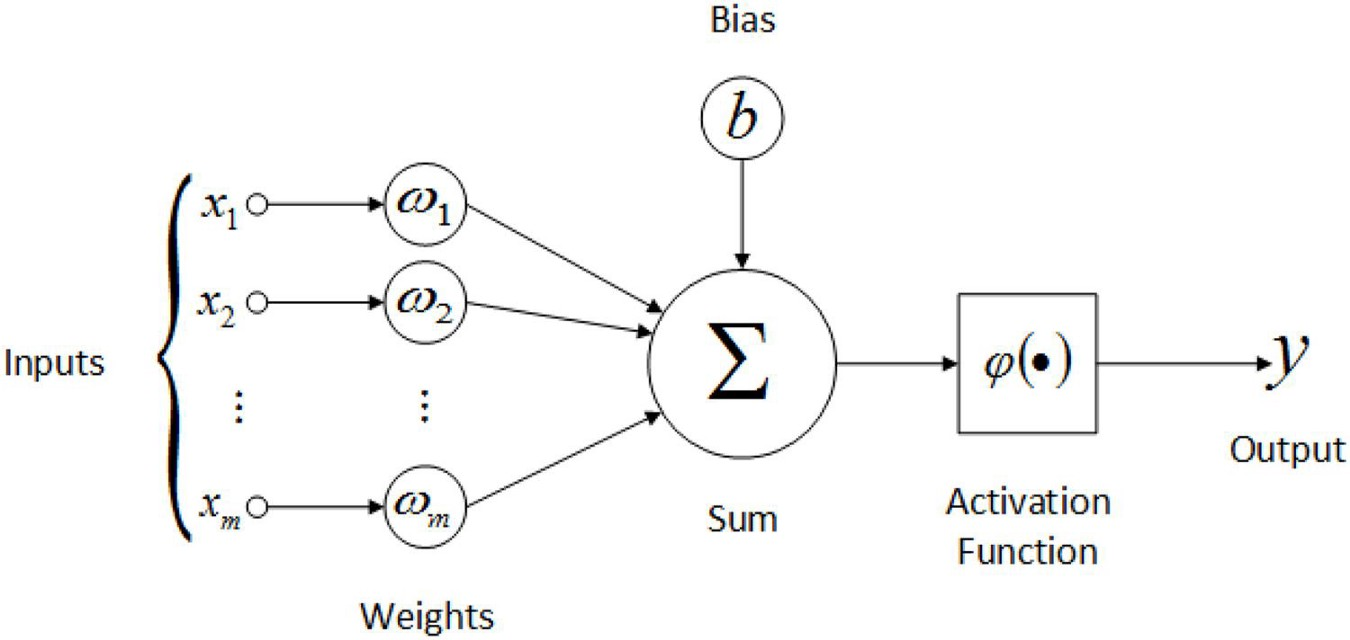
\includegraphics[height=3.8cm]{img/3_ML/neuron.jpg} \label{fig:mlp_a}}
    \subfigure[]{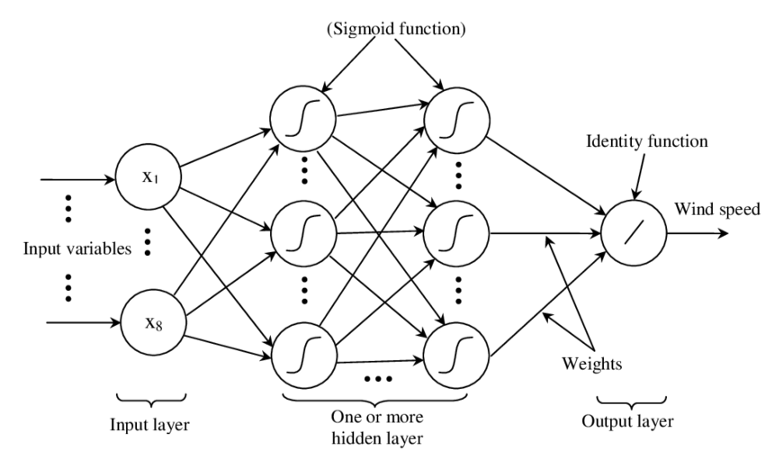
\includegraphics[height=3.8cm]{img/3_ML/MLP_1.png}  \label{fig:mlp_b}}
    \caption{the mathematical representation of neuron as the artificial neural network unit (a), and a sketch of a multilayer perceptron (b).}
    \label{fig:mlp}
\end{figure}
The~\Figure{\ref{fig:mlp_a}} shows a schematic representation of this artificial neuron: each of the $\bm{x}$ inputs is pre-multiplied by a proper weight $\bm{w}$, then the sum of the results, added with bias, is composed with a non-linear function $\varphi(\cdot)$. The output $y$ is then propagated to the next layer of neurons, as shown in the structure in~\Figure{\ref{fig:mlp_b}}, that represents the minimal solution for a \acs{MLP}. In this example the sigmoid activation function has been applied for all internal neurons, while a linear activation has been used for the final output.
From this perspective, the \acs{MLP} can learn to represent the output from a generic input by properly adjusting its weights $\bm{w_{ij}}$ to minimize a given \textit{loss function} in an optimization process.

The optimization is targeted to find the best functional fit for a set of input-output examples. So what we are doing at a very general level is tuning the weights to chase for an optimal configuration; but two complementary motivations determine what \textit{optimal} means in this context. On the one side we want the network to represent the target as exactly as possible, i.e. minimize the loss. But on the other side the network must be also \textbf{capable to generalize}, that is, when unknown inputs must be compared to the known, producing an output that is a kind of interpolation of learned values. However, good generalization and minimal reproduction error of the learned input-output pairs can become contradictory objectives.
A more detailed discussion is postponed to \cref{section:training_regularization}

In addition, the overall \acs{MLP} input-output map can be further seen as a non-linear regression, and the choice of the loss function is strictly related to the kind of output we are looking for. More precisely it corresponds to the probability distribution candidate we choose to fit the regression residuals. For a classification task, where the output of the network is a binary value identifying which class the input sample belongs to, the residuals are usually well described as a Bernulli distribution, and the loss function is usually the \textbf{binary cross entropy} (BCE). For a regression task, where we seek for a continuous output value, the loss is usually the \textbf{mean squared error} (MSE).
%
To give reason of these choices, two simple regression operators are hereafter presented.

\subsubsection{Linear regression}

The very basic linear regression model is a linear mapping from N-dimensional input features (or covariates) $\bm{x}$, to a one-dimensional target (or response) $y$, using the inputs, a set of weights (or regression coefficients) $\bm{w}$ and a bias offset $w_0$. The internal product of features and weights gives the equation of the fitter that in the linear form has the shape of a line in the N-dimensional space. The line is centered within the input data, while typically the probabilistic model assumes that the residuals can be described with a Gaussian shape of unknown variance $\sigma^2$. The model can be written as a predictor in the form:
\begin{equation}
    \hat{y} = \mu(\bm{x}) + \epsilon
\end{equation}
where $\mu(\bm{x}) = \expectation{y|\bm{x}}$:
\begin{equation}
     \mu(\bm{x}) = \transpose{\bm{w}}\bm{x} \qquad  \epsilon \in \mathcal{N}(0,\sigma^2)
\end{equation}
The first addendum is the \textit{linear predictor}, and the second addendum represents the error. To let the model fit also the bias the parameters and covariates array have been rewritten as follow:
\begin{equation}
    \bm{w} = [\hat{\bm{w}},w_0] \qquad \bm{x} = [\hat{x}, 1]
\end{equation}
Because we chose the noise to be Gaussian, the model can be rewritten as:
\begin{equation}
    p(y|\bm{x},\bm{w}) = \mathcal{N}(\mu(x), \sigma^2)
\end{equation}
This predictor represents a model (i.e. the N-dimensional line) that we want to center in such a way that the distance between data and the model output is minimal.
This can be done looking at $\bm{w}$ as the model parameters and imposing a \textit{likelihood} on the joint probability of the outputs of all the dataset samples. If the data set under analysis has cardinality $D$, the likelihood can be defined as:
\begin{align}
    \mathcal{L}(\bm{w}, y) &= \prod_i^D p(\bm{y}|\bm{w}) = \prod_i^D \mathcal{N}(\mu(x),\sigma^2) \\
    &= \frac{1}{(2\pi \sigma^2)^{\frac{D}{2}}} \exp \left[  -\frac{\sum_{i=1}^D (y_i-\mu(x)^2}{2\sigma^2} \right]
\end{align}
In maximization-minimization problems any objective function can be replaced with a monotone function that takes the original objective as its argument. A standard procedure is to look for the maximum of the log-likelihood that in turn corresponds to the minimum of the squared sum:
\begin{equation}
    \argmax{\bm{w}} \mathcal{L}(\bm{w},y) = \argmin{w} \sum_{i=1}^D (y_i - \transpose{\bm{w}}\bm{x})^2
\end{equation}
This is the same minimum of the \textbf{mean squared error}, hence the choice of this function as the \textit{loss}.

% It is worth noting that the likelihood appears to be
% this happens because we forced to consider the features with normal distribution and because being an exponential distribution it is also a conjugate prior for the likelihood, as it will described in the following.


\subsubsection{Logistic regression}

If we chose to implement a classifier instead, the output is best fitted by a Bernulli distribution:
\begin{equation}
    p(y|\bm{x},\bm{w}) = \mathrm{Ber}(y|\mu)
\end{equation}
in which this time for $\mu(\bm{x}) = \expectation{y|\bm{x}} = p(y=1|\bm{x},\bm{w})$ we chose a sigmoid function (also known as \textbf{logistic} or \textbf{logit} function):
\begin{equation}
    \mu(\bm{x}) = \mathrm{simg}(\transpose{\bm{w}}\bm{x}) = \frac{1}{1+e^{-\transpose{\bm{w}}\bm{x}}}
\end{equation}
At the same time the probability of the opposite outcome $p(y=0|\bm{x},\bm{w})$ is $1-\mu$, hence the likelihood for the joint probability on the dataset yields:
\begin{equation}
    \mathcal{L}(\bm{w}, y) = \prod_{i=1}^D p_i^{y_i}(1-p_i)^{1-y_i}
\end{equation}
And the log-likelihood is:
\begin{equation}
    \ln\mathcal{L} = \sum_{i=1}^D (y_i \ln p_i + (1-y_i)\ln(1-p_i))
    \label{eq:logistic_likelihood}
\end{equation}
Now, if we define $p_1 = p(y=1|\bm{x},\bm{w})$ and $p_0 = p(y=0|\bm{x},\bm{w})$, the cross entropy\footnote{information entropy is the average rate at which information is produced by a stochastic source of data.} of $p_0,p_1$ distributions is:
\begin{equation}
    H(p_1,p_0) = - \sum_i p_1(y_i) \ln p_0(y_i)
\end{equation}
Substituting $p_1$ and $p_0$ in equation~\eqref{eq:logistic_likelihood} reduces to the negative \textbf{cross entropy} function. Thus once again the maximum likelihood provides the correct definition of the loss function to chase optimum weights for the given distribution of errors.


%  _____ _____ ____  _   _      _                      _    
% |  ___|  ___|  _ \| \ | | ___| |___      _____  _ __| | __
% | |_  | |_  | | | |  \| |/ _ \ __\ \ /\ / / _ \| '__| |/ /
% |  _| |  _| | |_| | |\  |  __/ |_ \ V  V / (_) | |  |   < 
% |_|   |_|   |____/|_| \_|\___|\__| \_/\_/ \___/|_|  |_|\_\
%
\subsection{Statistical basis of the multilayer Perceptron}
\label{section:feedforward dense networks}

In the previous section two instances of regression operation have been presented. It has been also shown that the loss function used to optimize the network weights comes from maximizing the likelihood over the training data.
A further generalization of such regression operators can be provided making all posterior distributions to be in exponential family. The description of this unified representation, called \ac{GLM}, is proposed in appendix.

A feed forward neural network, also known as \ac{MLP}, is a composition of possibly non linear regression operations. For example if we set all activations to the sigmoid function, as in~\Figure{\ref{fig:mlp_b}}, \acs{MLP} can be seen as a chain of logistic regression stacked on top of each other. But the actual leading operation is the final layer that is again a regression for which a direct output error can be obtained, hence a loss can be chosen. For example it can be either a logistic or a linear regression depending whether we are looking for a general classification output (i.e. a probability function output for each of the classes in the classifier domain) or a regression output. 
For instance, looking at the simple two layers generic schema in~\Figure{\ref{fig:generic_mlp_a}}, and considering a linear regression for output, the model would be written like:
\begin{equation}
    p(y|\bm{x},\bm{\vartheta}) = \mathcal{N}\left(\transpose{\bm{w}}\bm{z(\bm{x}}), \sigma^2 \right)
    \label{eq:mlp_a}
\end{equation}
where all internal activation functions are represented by $\bm{z}(\bm{x})$ (the basis function expansion of the equivalent \acs{GLM} representation). This can be seen as a further non-linear response of all internal nodes:
\begin{equation}
    \bm{z}(\bm{x}) = \left[ g(\transpose{\bm{v}_1}\bm{x}), g(\transpose{\bm{v}_2}\bm{x}), ..., g(\transpose{\bm{v}_H}\bm{x})
    \right]
    \label{eq:mlp_b}
\end{equation}
and $\bm{\vartheta} = (\bm{w},\bm{v})$ collates all parameters.
In the single hidden layer example the deterministic function $g(\bm{x},\bm{v})$ is directly the internal nodes \textit{activation}, and it could be seen as the kernel of the basis function expansion of an equivalent \acs{GLM}. In this way we could think of the \acl{MLP} as a kernel machine~\cite{Scholkopf:1999:AKM:299094} where the kernel functions have been opportunely shaped to match the input data. 

% This parametrization on the kernel, by means of weights adjustment,  makes the \acl{MLP} an \ac{ABM}:
% \begin{equation}
%     f(\bm{x,\bm{\vartheta}}) = \transpose{\bm{w}}\bm{\phi}(\{1,\bm{x}\}, \bm{V})
% \end{equation}
% The generic basis function $\phi(\bm{x},\bm{V})$ must be trained on the dataset to make it "adapt" to the input statistics; while the entire parameter set that embrace the kernel is now: $\bm{\theta} = (\bm{w}, \bm{v})$ with $\bm{w} = [w_0, w_1, ..., w_M]$ and $\bm{v}_m = [v_{m1}, v_{m2}, ..., v_{mH}]$. The first set of parameters are the linear combination coefficients of the \ac{GLM}, and the second are the parametrization of the kernel. The unit appended to the input feature has been used to add the bias coefficient $w_0$.
%
\begin{figure}
    \centering
    \subfigure[]{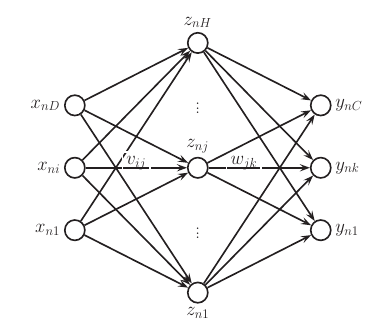
\includegraphics[height=6cm]{img/3_ML/MLP.png} \label{fig:generic_mlp_a}}
    \subfigure[]{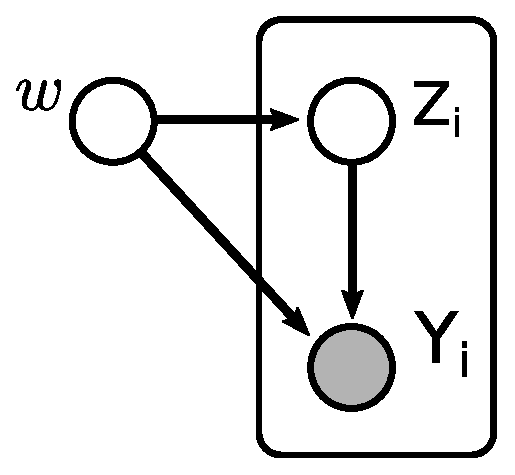
\includegraphics[height=3cm]{img/3_ML/MLP_PLATE.eps}}
    \caption{One hidden layer Feed Forward Neural Network (or equivalently the minimal Multi Layer Perceptron, seen as an Adaptive Basis Function Model (a), and the equivalent model in plate notation (b). }
    \label{fig:generic_mlp}
\end{figure}
%
The final \acl{GLM} applied can be constructed as usual in many different shapes, depending on the target type of inference we are interested in. If we look for a binary classification it appears as a logistic regression, i.e. the fit on the Bernoulli distribution of the sigmoid outputs:
\begin{equation}
    p(y|\bm{x}, \bm{\vartheta}) = \text{Ber}\left( y|\text{sigm}(\transpose{\bm{w}}\bm{z}(\bm{x}) \right)
\end{equation}
If we are looking for categorical classifier the correct GLM has to be distributed as:
\begin{equation}
    p(y|\bm{x}, \bm{\vartheta}) = \text{Cat}\left( y|\mathcal{S}(\transpose{\bm{w}}\bm{z}(\bm{x})) \right)
\end{equation}
where the \textit{Cat} distribution is the Multinulli and $\mathcal{S}$ stands for the support function of the input.

Furthermore the output description of the \acs{MLP} from \Figure{\ref{fig:generic_mlp_a}} is actually incomplete because in that schema the last layer regression is composed by multiple outputs. 
The proper extension to multiple output can be done by using a matrix composition: for instance the first regression example in \eqref{eq:mlp_a} can be more generally formulated as:
\begin{equation}
    p(\bm{y}|\bm{x}, \bm{w}) = \mathcal{N}\left( \bm{y}|\bm{W},\phi \right)
\end{equation}
where the probability has been shaped with the weights matrix $\bm{W}$ taking into account the possible MIMO configuration of the perceptron.
\begin{figure}
    \centering
    \subfigure[]{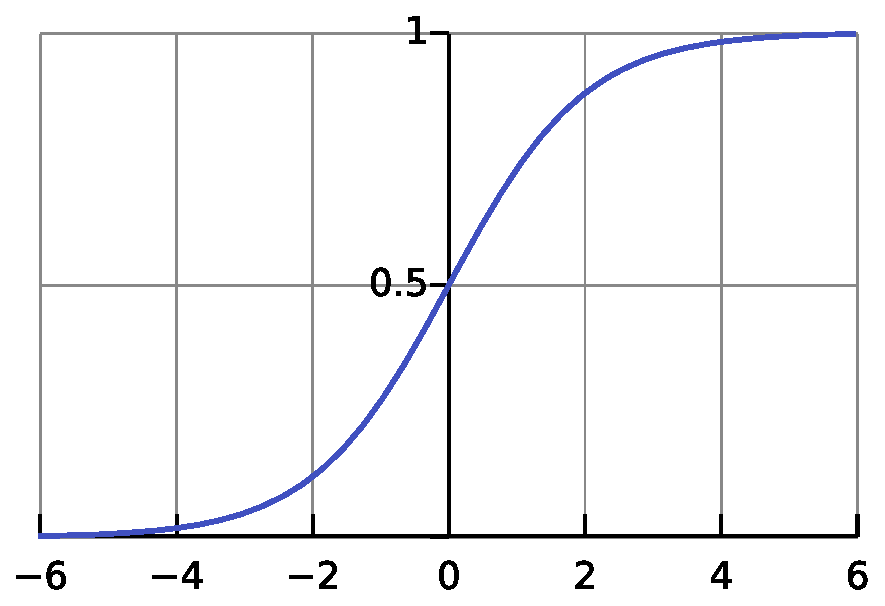
\includegraphics[height=3cm]{img/3_ML/Logistic-curve.eps} \label{fig:activations_logistic}}
    \subfigure[]{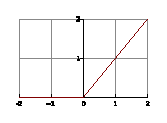
\includegraphics[height=3cm]{img/3_ML/Activation_rectified_linear.eps} \label{fig:activations_relu}}
    \caption{Two examples of activation functions: the logistic function, plotted in (a), defined as $y=\frac{1}{1+e^{-x}}$, and the rectified linear units (ReLU), shown in plot (b), defined as ${y = \text{max}: (0,x)}$. }
    \label{fig:activations}
\end{figure}
It is worth stressing the fact that a key factor for the activation function $g(\bm{x},\bm{v})$ is to be a non-linear operator, because the overall network would collapse into a large linear regression otherwise. Usually the activation is the logistic function $g(u) = \text{sigm}(u)$ or the recently much common flavors of the \textbf{rectified linear units} (ReLU) that provide a non linear activation with a minimal computational effort. The ReLU has the benefit of being scale invariant: $\textrm{max}(0,ax) = a\textrm{max}(0,x)$ for $ a \geq 0 $.
% FINIRE !!!!
% SHOW A FIGURE OF THE POSSIBLE ACTIVATION FUNCTIONS
% 
%
Feedforward neural networks early became a popular tool for non-linear regression and classification problems thanks to their simple mathematical expression and at the same time to their capability of easily adapting to any non-linear relation hidden within data. However this comes with the price that the network is trained to match the given inputs, thus it is actually prone to learn to represent this very set of data.
%
For this reason from a Bayesian perspective, the choice of neural network models can be viewed as the definition of a \textbf{prior over non-linear function}, while the learning process can be seen in terms of finding a posterior over those unknown function \cite{Polson_2017}. 
% SISTEMARE
As a bayes posterior the network can be then trained using a probabilistic approach, such as searching for the function parameters with maximum posterior probability (i.e. the Variadic Approach), or using Monte Carlo to sample directly from posterior. In particular this stochastic approach turns to provide a more robust representation in the case of generative networks, as it will be discussed in~\cref{section:VAE}.
%
%In the limit of standard networks with substantial scaling, Neal (1996) proved that the prior distribution over non-linear functions implied by the Bayesian neural network falls in a class of probability distributions known as Gaussian processes. 

% The hyperparameters of the neural network model
% determine the characteristic lengthscales of the Gaussian process. Neal’s ob-
% servation motivates the idea of discarding parameterized networks and working
% directly with Gaussian processes. Computations in which the parameters of
% the network are optimized are then replaced by simple matrix operations using
% the covariance matrix of the Gaussian process.


%% tell something about the cost function

% UNIVERSAL APPROXIMATION !!


%  _                _                          
% | |__   __ _  ___| | ___ __  _ __ ___  _ __  
% | '_ \ / _` |/ __| |/ / '_ \| '__/ _ \| '_ \ 
% | |_) | (_| | (__|   <| |_) | | | (_) | |_) |
% |_.__/ \__,_|\___|_|\_\ .__/|_|  \___/| .__/ 
%                       |_|             |_|    

\subsection{Optimization of parameters and the backpropagation algorithm}


If all the activations of \acs{MLP} had been linear functions, the model would have had a convex solution for the optimal weights; however the negative log-likelihood of a \acl{MLP} is a non-convex function of the parameters. It is nevertheless always possible to obtain a local maximum of the posterior probability locating the minimum of the loss function in a gradient-based optimization procedure. 
To proceed toward a descent path of the negative log-likelihood, a gradient vector is needed. This can be obtained in several ways, but it is a very common approach for NN to exploit the fact that the internal hidden units of a \acl{MLP} form a chain rule of calculus. The resulting algorithm is known as the \textbf{backpropagation}~\cite{NIPS2012_4824} and it will be briefly described in what follows, as it has been the method used in all the tests and results presented in this work. 

The backpropagation is a method to compute the variation of the computed loss with respect to a variation on the trainable variables in neuron units.
% so one could think that all hidden units as statistically described by internal states variables providing a stochastic version of the descent algorithm~\cite{rezende2014stochastic}; however in this brief description we will consider the hidden units as a part of the adaptive kernel of the \acl{MLP} as described, so that the optimum has only to be found among the gradients of all units function (i.e. the linear combination of coefficients and the activation function). 

To obtain a simple notation we will assume the model as it was presented in~\Figure{\ref{fig:generic_mlp_a}}: with just a single hidden layer. This will be indeed helpful to separate the \textit{pre-synaptic} and \textit{post-synaptic} entities of neurons, that are values of the signal passing through, before and after we apply the non-linearity of the activation function. Let $\bm{x}_n$ be the n'th input, $\bm{a}_n = \bm{V}\bm{x}_n$ the \textit{pre-synaptic} hidden layer, and $\bm{z}_n = g(\bm{a}_n)$ the \textit{post-synaptic} hidden layer, where $g$ is any transfer function. 
For the activation, as already discussed, several non-linear function is commonly used. The classical literature presents $g(a) = sigm(a)$, or equivalently $g(a) = tanh(a)$, but we also stated that a common modern solution is to exploit the ReLU or Leaky-ReLU functions. 
We will now consider the model as presented in \Equation{\ref{eq:mlp_a}}; the pre and the post synaptic outputs can be divided as: $\bm{b}_n = \bm{W}\bm{z}_n$ pre-synaptic output, and $\hat{\bm{y}}_n = h(\bm{b}_n)$ the post-synaptic output. In the second term we also represented the non linear effect of the \acl{GLM} canonical link function as $h$.

The gradient descent method involves calculating the derivative of the loss function with respect to the weights of the network. This is normally done using backpropagation. Assuming one output neuron, the squared error function is:
\begin{equation}
    E = L(t, y)
\end{equation}
where $E$ is the loss choice for the the output $y$ and target value $t$.
For each neuron $j$, its output $y_j$ is defined as
\begin{equation}
    y_j = \varphi\left(\sum_{k=1}^n w_{kj}y_k\right),
\end{equation}
%
The partial derivative of the error with respect to a weight $w_{ij}$ can be calculated as:
\begin{equation}
    \pdv{E}{w_{ij}} = \pdv{E}{y_j}\pdv{y_j}{w_{ij}} = \pdv{E}{y_j}\pdv{y_j}{\mu_j}\pdv{\mu_j}{w_{ij}}
\end{equation}
%
In the last factor of the right-hand side of the above, only one term in the sum, $\mu_j$, depends on $w_{ij}$, so that
%
\begin{equation}
    \pdv{\mu_j}{w_{ij}} = \pdv{}{w_{ij}}\left( \sum_{k=1}^n w_{ij}\mu_k \right) = \pdv{}{w_{ij}}w_{ij}\mu_i = \mu_i
\end{equation}
%
If the neuron is in the first layer after the input layer, $y_i$ is just $x_i$.
The derivative of the output of neuron $j$ with respect to its input is simply the partial derivative of the activation function:
%
\begin{equation}
    \pdv{y_j}{\mu_j} = \pdv{\varphi(\mu_j)}{\mu_j}
\end{equation}
%
which for instance for the logistic activation function case is:
\begin{equation}
    \pdv{y_j}{\mu_j} = \pdv{}{\mu_j} \varphi(\mu_j) = \varphi(\mu_j)(1 - \varphi(\mu_j))
\end{equation}
where the logistic activation is defined as:
\begin{equation}
    \varphi(z) = \frac 1 {1+e^{-z}}
\end{equation}
and its derivative is trivial:
\begin{equation}
    \frac {d \varphi(z)}{d z} = \varphi(z)(1-\varphi(z)) 
\end{equation}
%
This is the reason why backpropagation requires the activation function to be differentiable.
A recursive expression for the derivative can be obtained:
\begin{equation}
    \pdv{E}{y_j} = \sum_{l \in L} \left( \pdv{E}{\mu_l} \pdv{\mu_l}{y_j} \right) 
    = \sum_{l \in L} \left( \pdv{E}{y_l} \pdv{y_l}{\mu_l} \pdv{\mu_l}{y_j} \right)
    = \sum_{l \in L} \left( \pdv{E}{y_l} \pdv{y_l}{\mu_l} w_{jl} \right)
\end{equation}
%
Therefore, the derivative with respect to $y_j$ can be calculated if all the derivatives with respect to the outputs $y_l$ of the next layer are known.
\begin{equation}
    \pdv{E}{w_{ij}} = \pdv{E}{y_y} \pdv{y_j}{\mu_j} \pdv{\mu_j}{w_{ij}} = \pdv{E}{y_j} \pdv{y_j}{\mu_j} y_j = y_i \delta_j
\end{equation}
defining $\delta_j$ as:
\begin{equation}
    \delta_j = \pdv{E}{y_j} \pdv{y_j}{\mu_j}
\end{equation}
%
Hence for an output neuron:
\begin{equation}
    \pdv{L(y_j,t)}{y_j} \frac{d\varphi(\mu_j)}{d \mu_j}
\end{equation}
%
and for a inner neuron:
\begin{equation}
    \left( \sum_{l \in L}w_jl \delta_l \right)  \frac{d\varphi(\mu_j)}{d \mu_j}
\end{equation}
%
and all updates can be made proportional to $\delta_j$ like:
\begin{equation}
    \Delta w_{ij} = -\alpha \pdv{E}{w_{ij}} = -\alpha y_i \delta_j
\end{equation}


%In the regression case of \acl{GLM} the negative log-likelihood appears as the \textbf{mean squared error} of the signal that passed through the network with the ground truth:
% \begin{equation}
%     J(\bm{\theta}) = -\sum_n\sum_k \left(\hat{y}_{nk}(\bm{\theta}) - y_{nk}\right)^2
% \end{equation}
% In the classification case the negative log-likelihood assumes the typical form of the \textbf{cross entropy} between the reconstruction output and the actual real class of each sample:
% \begin{equation}
%     J(\bm{\theta}) = -\sum_n\sum_k y_{nk} \log \hat{y}_{nk}(\bm{\theta})
% \end{equation}
% %
% Let us start by considering the output layer weights from the MLP:
% \begin{equation}
%     \nabla_{\bm{w}_k} J_n = \pdv{J_n}{b_{nk}} b_{nk} = \pdv{J_n}{b_{nk}} \bm{z}_n
% \end{equation}
% where $b_{nk} = \transpose{\bm{w}_k}\bm{z}_n$. Considering all the chained relations, it can be shown ( see GLM ML ) that the the derivative can be set to:
% \begin{equation}
%     \pdv{J_n}{b_{nk}} = ( \hat{y}_{nk} - y_{nk} ) \triangleq \delta_{nk}^w
% \end{equation}
% and the overall gradient with respect to the output signal is:
% \begin{equation}
%     \nabla_{\bm{w}_k} J_n = \delta_{nk}^w \bm{z}_n
% \end{equation}
% A similar procedure can be also applied to the input layer:
% \begin{equation}
%     \pdv{J_n}{a_{nj}} = \sum_{k=1}^K \pdv{J_n}{b_{nk}}\pdv{b_{nk}}{a_{nj}} 
%     \triangleq \sum_{k=1}^K \delta_{nk}^w \pdv{b_{nk}}{a_{nj}}
% \end{equation}
% Now we introduce the actication function at the input of the link function, so from the defined $b_{nk}$ as:
% \begin{equation}
%     b_{nk} = \sum_j w_{kj} g( a_{nj} )
% \end{equation}
% the derivative becomes:
% \begin{equation}
%     \pdv{b_{nk}}{a_{jk}} = w_{kj} g^\prime(a_{nj})
% \end{equation}
% The derivative of the activation function varies for the specific case; for example:
% \begin{align*}
%     & \pdv{}{a} \tanh(a) = 1-\tanh^2(a) \\
%     & \pdv{}{a} \text{sigm}(a) = \text{sigm}(a)(1-\text{sigm}(a))
% \end{align*}
% Hence:
% \begin{equation}
%     \delta_{nj}^v = \sum_{k=1}^K \delta_{nk}^w w_{kj} g^{\prime}(a_{nj})
%     \label{eq:backprop_error}
% \end{equation}
% Putting it all together, we can compute all the gradients as follows: we first perform a forward pass to compute $a_n$ , $z_n$ , $b_n$ and $\hat{y}_n$. We then compute the error for the output layer, $\delta_n^{(2)} = \hat{y}_n - y_n$, which we pass backwards through $\bm{W}$ using \eqref{eq:backprop_error} to compute the error for the hidden layer $\delta_n^{(1)}$. We then compute the overall gradient as follows:
% \begin{equation}
%     \nabla_{\bm{\theta}} J(\bm{\theta}) = \sum_n \left[ \bm{\delta}_n^v \bm{x}_n, \bm{\delta}_n^w \bm{z}_n \right]
% \end{equation}

It is also quite straightforward to see that the parameters are not uniquely identifiable. For example, we can change the sign of the weights going into one of the hidden units, while changing the sign of all the weights out of it; these composed effects cancel. Similarly, we can change the identity of the hidden units without affecting the likelihood. 
In addition, there may be local minima due to the general non-convexity of the log-likelihood. Although this can become a serious problem in some situations, with enough data information these local optima are often quite “shallow” and the simple stochastic optimization methods can reach the global optimal value of the parameters. In addition further optimized descent variants can be also considered that fall in the category of regularization methods. 

%                       _            _          _   _             
%  _ __ ___  __ _ _   _| | __ _ _ __(_)______ _| |_(_) ___  _ __  
% | '__/ _ \/ _` | | | | |/ _` | '__| |_  / _` | __| |/ _ \| '_ \ 
% | | |  __/ (_| | |_| | | (_| | |  | |/ / (_| | |_| | (_) | | | |
% |_|  \___|\__, |\__,_|_|\__,_|_|  |_/___\__,_|\__|_|\___/|_| |_|
%           |___/                                                 

\subsection{Regularization}
\label{section:training_regularization}
Both in the introductory chapter and the previous section the general concept of generalization and fitting of the network has been introduced. A more detailed description of the phenomenon and the approach used to provide a solution are described in the following.
The operation of making the network "generalizing" well over unknown inputs is generally referred to as the \textbf{regularization}. This is quite a complex argument though that spans across different aspects of the network engineering, such as the dataset organization, the activation selection, the network topology shaping, the internal layers operations, etc. 

Hereafter two main kinds of regularization will be described: the \textbf{training regularization} as all the action that play during training, for example by reordering dataset, changing learning rate, or adding operands to the loss function; and the \textbf{network regularization} as all possible permanent modifications to the network that continue to hold also after the training is concluded.
Some regularization techniques, as the ones just exposed, have been effectively used during the tests presented in this work so they will be briefly presented in the next sections.

\subsubsection{Adaptive moment optimization}
In the previous section the general approach known as the backpropagation algorithm that provides the gradient to search for maximum likelihood, or equivalently the minimum loss function, has been explained. 
The backpropagation algorithm outputs a value for the parameters update during the iterative steps of the gradient descent; this update is then applied through a learning factor that acts as a update multiplier. The aim is to provide a good global minimum of the loss function.
Usually this implies a variation of the learning rate during the training epochs, for example it undergoes a reduction on the plateau of the learning curve simulating a sort of annealing of the parameters updates; a typical solution is to apply a simple callback function that uses the epoch number and the loss values to iteratively update the learning factor.
Although this simple principle appears quite easy, and it is already provided by some frameworks such as \textit{keras}, it presents some difficulties such as the fact that it can't be effectively applied on the actual plateau but only at fixed times (i.e. end of epoch) during training; also it does not automatically account the possible noise associated to the instant loss value of a poorly regularized training.

Another method that recently gained a lot of attention was presented by Diederik Kingma (2015) called \textbf{Adam} (a contraction for "\textit{adaptive moment estimation}")~\cite{kingma2014adam}. This specific formulation can be used instead of the classical stochastic gradient descent procedure to update network weights based on the training dataset; it computes individual adaptive learning rates for parameters exploiting the estimates of first and second order moments of the gradients. 
We choose to apply this method during the tests performed, thanks to the computational efficiency and the little memory required, and because it appears to be very flexible where the dataset used leads to noisy gradients.
Specifically, the algorithm calculates an exponential moving average of both the gradient value and its squared, and further global parameters $\beta_1$ and $\beta_2$ control the decay rates of these moving averages. 
The initial value of the moving averages and the control parameters are usually close to 1.0 resulting in a bias of moment estimates towards zero. This bias is overcome by first calculating the biased estimates before, and then calculating bias-corrected estimates.
If we set the computed gradients of the backpropagation algorithm as:
\begin{equation}
    g_t = \nabla_{\bm{\theta}} f_t(\bm{\theta_{t-1}})
\end{equation}
where $\bm{\theta}$ represents the set of the learnable parameters, meaning the network parameters that will be adjusted during learning, the estimates of the moments is:
\begin{align}
    & m_t = \frac{\beta_1 m_{t-1} + (1 - \beta_1) g_t  }{1-\beta_1} \\
    & v_t = \frac{\beta_2 v_{t-1} + (1 - \beta_2) g_t^2}{1-\beta_2}
\end{align}
the update of parameters is applied as:
\begin{equation}
    \bm{\theta}_t = \bm{\theta}_{t-1} - \alpha \left( \frac{m_t}{v_t^\frac{1}{2} + \epsilon} \right)
\end{equation}

\subsubsection{Convolutional layers}
Multilayer perceptrons (MLPs) are fully connected networks and therefore every neuron in a given layer is connected to all the neurons in the previous one. A problem in this topology is that MLP are prone to overfit data, On the other side, Convolutional Neural Networks (CNNs) use a simplified network structure where every neuron in a given layer is connected only to a subset of neurons in the previous one, exploiting a structure that is similar to the neurons in animal retina. 

% The previous sections explained how the \ac{ABM} hidden units are able to learn non-linear combinations of the original inputs; this is generally referred as the process of \textbf{feature extraction}. In this context the extraction means that the hidden units provide the tempered features for the input to the final \ac{GLM}. 
% %
% Moreover, thanks to the properties of the fully connected network and in particular to the universal approximation theorem, this approach proves to be particularly effective, specially for problems where the original input covariates are not very individually informative. 
% Although the real power NNs is acting out the non-linear relations on input signals, for a task where there is a strong sequential correlation among covariates extracting “higher order” features with fully connected neurons is less important.
% %
% The convolutional layers - the basis of famous \ac{CNN} models like AlexNet~\cite{Krizhevsky:2012:ICD:2999134.2999257}, GoogleNet/inception~\cite{7298594} -, are yet another example of this concept, thus it should not be surprising fact that it actually behave like a means of network regularization.

% As what has been just presented about Adam optimizer, typical ways of regularization include adding some form of magnitude measurement of weights to the loss function. However this is not the sole way to make the network output more general; \acl{CNN} networks take a different approach for regularization: they take advantage of the hierarchical pattern within the data to represent complex patterns using smaller and simpler ones. 
In more detail convolutional networks are simply neural networks that use convolution in place of general matrix multiplication in at least one of their hidden layers.
For a 2D-image for instance the \textbf{convolutional layers} have hidden units with \textbf{local receptive field}, where the learning parameters (i.e. the $\bm{V}$ matrix of convolution layers) are tied together in the convolution kernel and thus shared across the image. Intuitively, the effect of such spatial relation is that any useful features that are “discovered” in a portion
of the image can be re-used everywhere else without having to be learned independently. The resulting networks then exhibit a translation invariance - they are also referred as \textbf{space invariant artificial neural networks} (SIANN) - meaning they can recognize patterns no matter where they are occurring within the input.
The same holds for 1D-signals too, as a similar spatial relation can be made explicit as well.

So convolutional layers are a form of regularization in the sense that, while for a \ac{MLP} the fully connected network (where each neuron in one layer is connected to all neurons in the next) makes it prone to overfit data, in \ac{CNN} the effect of sharing parameters along the features could eventually compress the network complexity. Or, equivalently, a small network with convolutional layers, thanks to external assumptions on the nature of the data, can act like a bigger one with a more complex behavior. CNNs are now widely used in feature detection from images and represent a promising approach for plasma diagnostics based on camera images.% METTERE FIGURA DI CONVOLUTIONAL LAYERS!! %%
%
% In addition it will be shown - and is the actual main target of the present study - how the very deep joint relations among features can be easily managed by \ac{DNN} without handling the complex models that drive the experimental outcomes; but that we can also make the frequentists approach (i.e. stochastic modeling) closer to the physical and theoretical aspects of experiments with regularization.

\subsubsection{Dropouts}
Being a stochastic process, the NN training is also prone to find different solutions to the same problem, depending for example on the initial conditions. This eventually leads to possible local minima. 
\textit{Dropout} is another network regularization method that makes the training process behave like it were contemporaneously training a large set of neural networks with different architectures in parallel~\cite{Srivastava:2014:DSW:2627435.2670313}.
By dropping a unit out, we mean temporarily removing it from the network, along with all its incoming and outgoing connections.
So, during the training, some number of layer outputs are randomly ignored or, as the name says, they are “dropped out”. This has the effect that in each attempt the actual layer that plays in optimization looks like a layer with a different number of nodes and connectivity with respect to the previous one. In last effect, each update to a layer during training is performed with a different “view” of the configuration as the overall network was a different one.

% \begin{lstlisting}[language=Python, caption=Dropout layer code example (from Tensorflow 2.0)]
% @tf_export("nn.dropout", v1=[])
% def dropout_v2(x, rate, noise_shape=None, seed=None, name=None):
%     [...]
%     random_tensor = random_ops.random_uniform( noise_shape, seed=seed, dtype=x.dtype ) 
%     keep_prob = 1 - rate 
%     scale = 1 / keep_prob
%     keep_mask = random_tensor >= rate
%     return = x * scale * math_ops.cast(keep_mask, x.dtype)
% \end{lstlisting}

\subsubsection{Batch normalization}
A further method to increase the stability (read generalization) of a neural network is the \textit{batch normalization}~\cite{ioffe2015batch} layer. It normalizes the output of the previous activation by subtracting the mean and dividing by the standard deviation computed on the mini-batch (mini batches represent subsets sets of the training set, usually randomly picked).  However, after this shift and scale of the activation output - that are operated by some randomly initialized parameters - the weights in the next layer may be no longer optimal. The optimization process so tends to destroy this normalization if it move the output away from the loss function minimum.
As stated, the batch normalization adds two further trainable parameters: the normalized output is multiplied by a “standard deviation” parameter ( $\gamma$ ) and added to a “mean” parameter ( $\beta$ ). 
% In other words, batch normalization lets stochastic gradient do the de-normalization by changing only these two weights for each activation, instead of losing the stability of the network by changing all the weights.
Considering a given hidden layer in the NN, we compute the moments of the hidden layers outputs over the mini-batch as:
\begin{align*}
    & {\mu_l}_{\text{BN}} = \expectation{\bm\phi_l(\bm{x})} \\
    & {\sigma^2_l}_{\text{BN}} = \expectation{ (\bm\phi_l(\bm{x}) - {\mu_l}_{\text{BN}})^2 }
\end{align*}
where $\phi_l(x_i)$ is the i-th activation output of the l-th layer when BN is applied.
Then we apply the normalization:
\begin{equation}
    \hat{x_i} = \frac{x_i - {\mu_l}_{\text{BN}}}{ {\sigma_l}_{\text{BN}} + \epsilon }
\end{equation}
Finally the scale and shift operation is:
\begin{equation}
    y_i = \gamma \hat x_i + \beta
\end{equation}
Where $\gamma$ and $\beta$ are two added learnable parameters, that partecipate to the overall (differentiable) network transfer function and that are updated during the gradient descend learning phase. When the network has been trained this way, it is necessary to perform the normalization during network recall and in this case a global mean and standard deviation must be computed considering the actual set of inputs. Alternatively an exponential weighted “moving average” can be used to update population mean and variance. \\
One effect of the Batch Normalization is to generally increase the training speed as a higher learning rate can be used; this happens because batch normalization constrains activation functions output to a limited support. 

It also reduces over-fitting, because, similarly to the Dropout, it adds a noise to each hidden neuron activation. Therefore, if we use batch normalization, we will use less or even no dropout, which is a good thing, because we are not going to lose a lot of information. However the two effects are not interchangeable.
%
% It is also quite straightforward to see that this kind of regularization layer, as well as the convolutional layer, is a \textbf{network regularizer} thus it must be always kept in the model, even after the end of the training. This represent in a way a limitation of the expression capability because it must be implemented in every running software or hardware support chosen for the final deployment of the network. This could seem a slight drawback because the overall networks grows in parameters, however, aside of the benefit of the regularization, the layer bias coefficient of the linear combination can (an should) be removed because the bias effect is wiped out by the output mean shift.

\subsubsection{Activity regularization}
Activity regularization is instead a \textbf{training regularization} that provides a way to encourage a neural network to learn sparse features or internal representations of raw observations.
It is quite common to push sparsity of representation in autoencoders as we will see in few paragraphs, although the approach can be used also generally both in reducing over-fitting and improving network generalization.

The activity regularization acts on the parameters, i.e. the amplitude of the learned weights, working on the assumption that smaller weights tend to generate simpler models and thus they help to avoid over-fitting. We will present here two kinds of such activity regularizers named L1-norm (Lasso regularizer) and L2-norm (Ridge regularizer). Both methods basically add a penalty term in the loss function that tends to reduce the weights of the network. \\
The penalty term used in Lasso regularization is:
\begin{equation}
    L_1 \triangleq \lambda_1 \sum_{i=1}^{H_l} \left| v_i \right|
\end{equation}
In L2 regularization, the penalty term is the sum of square of all feature weights:
\begin{equation}
    L_2 \triangleq \lambda_2 \sum_{i=1}^{H_l} v_i^2
\end{equation}
At the end the overall Loss is composed by the target loss, \textit{mse} for instance, and the sum of all layer losses:
\begin{equation}
    L(x,y) = \sum_{i=1}^N (y_i - \transpose{\bm{w}}\bm{z_i}(\bm{x}))^2 + \lambda_1 \sum_{j=1}^{L1} L_1(x_i,y_i)_j + \lambda_2 \sum_{k=1}^{L2} L_2(x_i,y_i)_k
\end{equation}

These activity regularizers are only affecting the loss and thus they only pertain on training, so they are \textit{training regularizers} and shall not be eventually deployed in a trained network.
% \begin{lstlisting}[language=Python, caption=activity L1L2 regularizer in keras (tf 2.0)]
% @keras_export('keras.regularizers.L1L2')
% class L1L2(Regularizer):
%   def __call__(self, x):
%     if not self.l1 and not self.l2:
%       return K.constant(0.)
%     regularization = 0.
%     if self.l1:
%       regularization += self.l1 * math_ops.reduce_sum(math_ops.abs(x))
%     if self.l2:
%       regularization += self.l2 * math_ops.reduce_sum(math_ops.square(x))
%     return regularization
% \end{lstlisting}



%  _   _ _   _ ____  _   _ ____  _____ ______     _____ ____  _____ ____  
% | | | | \ | / ___|| | | |  _ \| ____|  _ \ \   / /_ _/ ___|| ____|  _ \ 
% | | | |  \| \___ \| | | | |_) |  _| | |_) \ \ / / | |\___ \|  _| | | | |
% | |_| | |\  |___) | |_| |  __/| |___|  _ < \ V /  | | ___) | |___| |_| |
%  \___/|_| \_|____/ \___/|_|   |_____|_| \_\ \_/  |___|____/|_____|____/ 

\section{Unsupervised learning: Generative modeling}
%
"Generative modeling" is a broad area of machine learning that deals with probability distribution models, defined on data points $p(\bm{x})$ in a potentially large $X$ space. For example, images are a popular type of data for which we could create generative models. Each "data point" (image) has thousands or millions of dimensions (pixels) and the work of the generative model is in some way capturing the dependencies between the pixels. What exactly "capturing" these dependencies means depends on what we want to do with such models.

In first approximation the unsupervised approach aims at describing the source distribution $p(x)$.
For example, in the case of images passing through convolutional networks, the $\bm{x}$ values that look like real images should have a high probability, while images that look like random noise should present low probability in the distribution. However, models like this are not necessarily useful: knowing that an image is unlikely does not help us synthesize what is likely. 

More often we worry about producing more examples similar to those already present in a database, but not exactly the same. We could start with a database of raw images and synthesize new and unseen images. We could take a database of 3D models of something like plants and produce more to fill a forest in a video game. We could take handwritten text and try to produce more handwritten text. Tools like this could actually be useful for graphs. We can formalize this configuration by saying that we get X examples distributed according to an unknown $p(x)$ distribution and our goal is to learn a model from which we can obtain samples that are as similar as possible to $p(x)$.

Among the possible solutions to perform the $p(x)$ description the very general approach consists on the dimensionality reduction of the input domain, and we can distinguish two main categories. A first category exploits a deterministic algorithm to generate a more compact representation of data, for example the clustering methods like k-means~\cite{Kanungo00anefficient} and t-SNE~\cite{vanDerMaaten2008}, or the latent embedding such as LLE~\cite{Roweis2000} and Autoencodes~\cite{Goodfellow-et-al-2016}.
The methods in the second category, on the other hand, exploit a stochastic approach and a variational training; among them, Deep Belief Networks~\cite{hinton_DBN}, \ac{VAE}~\cite{DBLP:journals/corr/KingmaW13}~\cite{DBLP:conf/iclr/2014}, and GAN~\cite{Goodfellow:2014:GAN:2969033.2969125}.

\subsubsection{Autoencoders}

One of the most common approaches to unsupervised learning, and the method exploited in the present work, is the class of generative models called Autoencoders.
An autoencoder can be defined as a neural network whose primary purpose is to learn the underlying manifold or the feature space in the dataset. The network structure is symmetric, the input and output layers are identical, because the autoencoder tries to reconstruct an exact match of the inputs. Unlike other nonlinear dimension reduction methods, the autoencoders are not based on a single property of the data like distance (k-means, t-SNE), or the data topology (PCA, LLE). An autoencoder generally consists of two parts: an encoder which transforms the input to a hidden code, and a decoder which reconstructs the input from the hidden code. The main feature is a reduced dimension on at least one of the hidden layers, that is the output of the decoder. This induces the network to extract the main representative features in the encoder part, and at the same time provides a network to regenerate the input from those extracted features.
\begin{figure}[h]
    \centering
    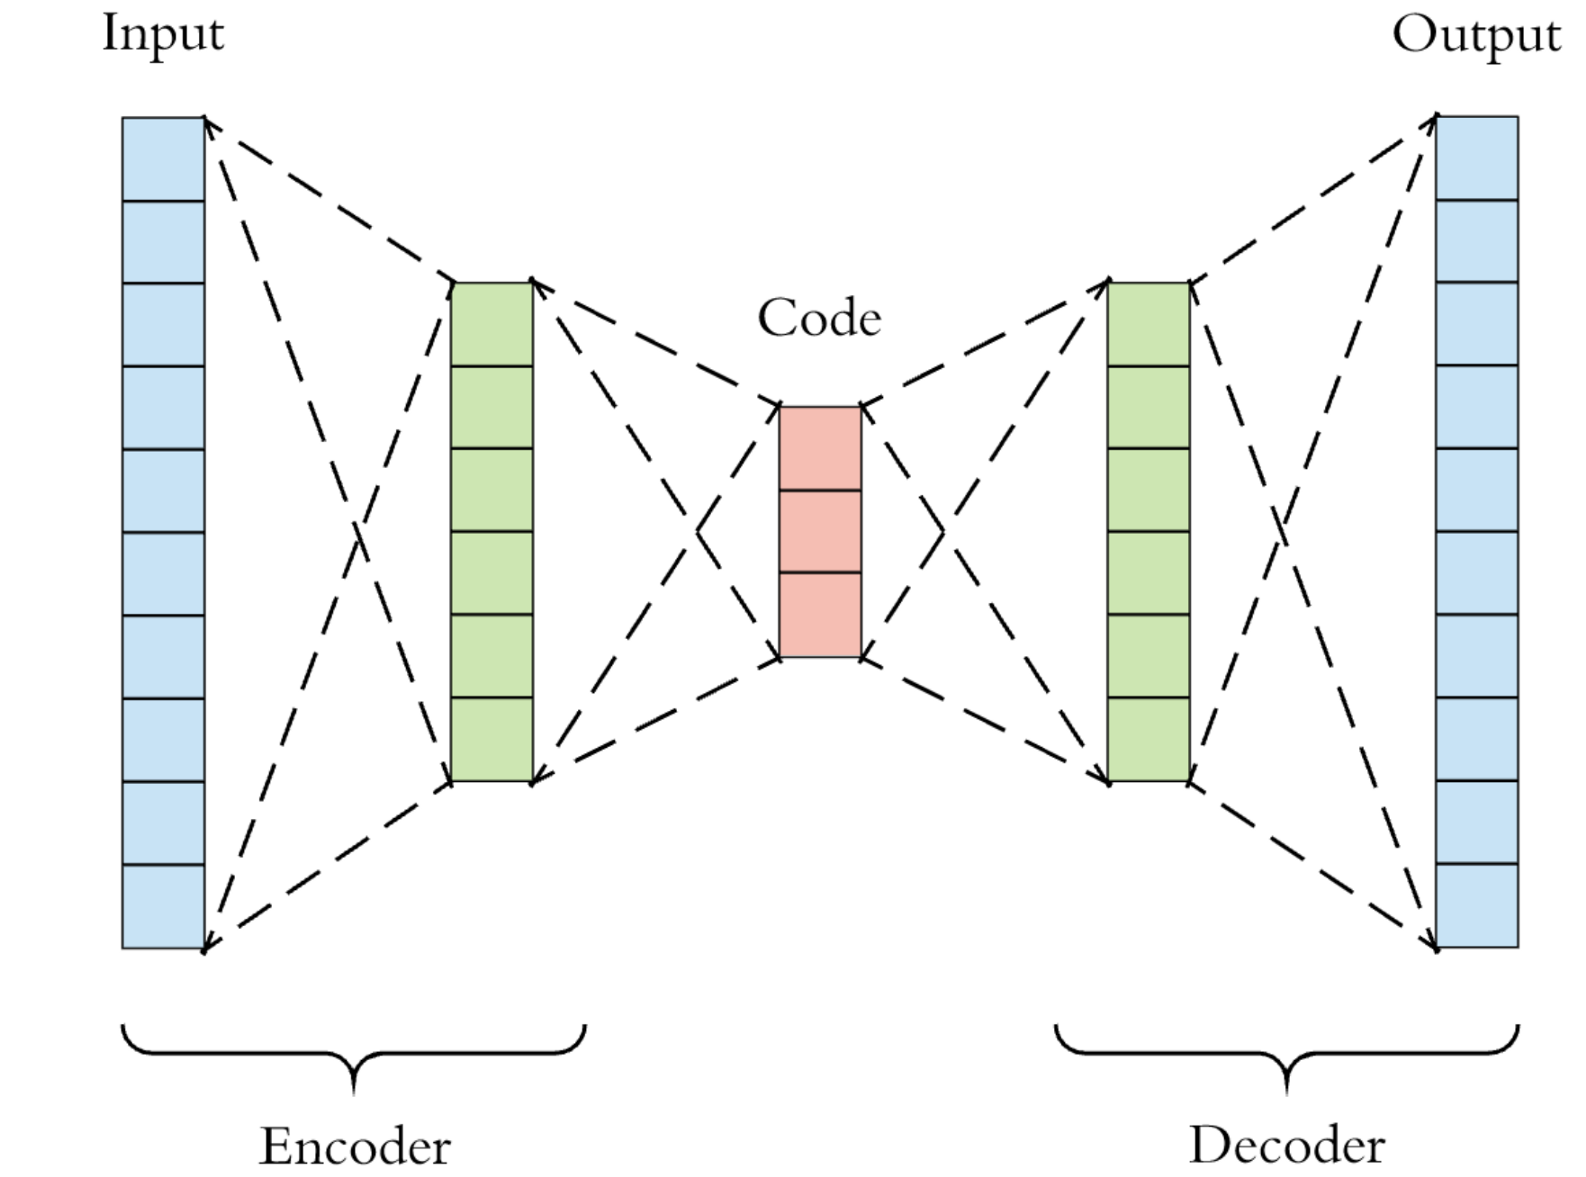
\includegraphics[height=5cm]{img/3_ML/Autoencoder.png}
    \caption{The basic schematic representation of the Autoencoder internal network organization, in which a first encoder extracts a code from input features with a lower dimensionality, then a decoder generates an output from code that tends to be similar to the given input. }
    \label{fig:autoencoder}
\end{figure}
In~\Figure{\ref{fig:autoencoder}} a simple schematic view of the Autoencoder internal structure has been given, showing the inner bottleneck that performs the dimensionality reduction.
% Instead of providing a detailed description of the Autoencodes here, it will be done in the following section through the explanation of their variational version that is the actual formulation we used to produce our results.


% \subsection{Latent Variables Models}

% Before entering in the Variational Autoencoder details, it is useful to introduce the basic structure of the bayesian networks, that is the fundamental structure that subtends \acs{VAE}s. 

% As it has been shown that a general approach to obtain the regression of a single variable given its conditional probability in the supervised training. Suppose now that we are observing a set of multiple correlated variables where the correlation extends from one variable to another in a chain of dependencies. This becomes a stochastic model describing a sequence of possible values for the variables in which the probability of each event depends on the state of the others.



% %



% It has been already presented that directed joint probability distributions. The basic idea is to graph all conditional dependencies among variables by adding an edge between each of the linked pairs. 
% We also saw as an alternative approach, assuming that the observed variables are correlated because they arise from a hidden common “cause”, that the model can be added with hidden variables (i.e. \textbf{latent variable models}).
% Such expanded models are actually harder to fit because for the latent variables we need to infer their distribution as well as than models with no latent variables.
% %
% \begin{figure}
%     \centering
%     \subfigure[]{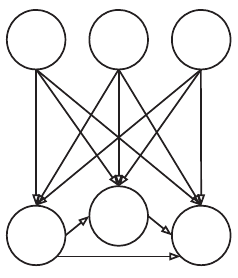
\includegraphics[height=3cm]{img/3_ML/mixed_model_FCL.png} \label{img:ML_mm_flc}}
%     \subfigure[]{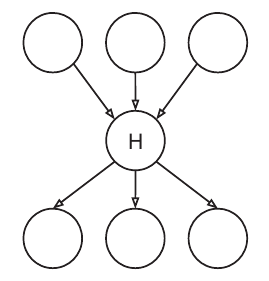
\includegraphics[height=3cm]{img/3_ML/mixed_model_LVM.png} \label{img:ML_mm_lvm}}
%     \caption{Connections topology between the fully connected bayes network, where all conditional probabilities are explicitly assigned between each pair of the layers nodes  (a), and the same model with a latent \textit{hidden} variable inserted between layers to represent conditional probabilities (b). }
%     \label{fig:mixture_models}
% \end{figure}
% %
% However once the \acs{LVM} is built the total number of parameters is significantly reduced in respect with the same model that directly represent correlation in the visible space. 



% \subsubsection{linear factor analysis}
% \label{linear factor analysis}
% % RR
% One problem with mixture models is that they only use a single latent variable to generate the
% observations. In particular, each observation can only come from one of K prototypes. One can
% think of a mixture model as using K hidden binary variables, representing a one-hot encoding
% of the cluster identity. But because these variables are mutually exclusive, the model is still
% limited in its representational power.
% An alternative is to use a vector of real-valued latent variables, $z_i \in R_L$ . The simplest prior
% to use is a Gaussian:


% If the observations are also continuous, so $x_i \in R_D$ , we may use a Gaussian for the likelihood.
% Just as in linear regression, we will assume the mean is a linear function of the (hidden) inputs,
% thus yielding



% The training procedure of this type of models has been a long-standing problem in machine learning; and, in general, most approaches have had three major drawbacks: they may require strong assumptions about the data structure, they could make serious approximations leading to sub-optimal patterns, or they could rely on computationally expensive inference procedures like Markov Chain Monte Carlo integration. More recently the community made tremendous progress in training neural networks, as for instance the powerful approximators of functions via backpropagation~\cite{NIPS2012_4824}. These advances gave rise to promising frameworks that can use function approximators based on backpropagation to build generative models. One of the most popular frameworks of this type is the Variable Autoencoder \cite{} that will be presented in the following, and will be the main actor of this study. The assumptions of this model are weak and the training is fast through backpropagation. VAEs make an approximation, but the error introduced by this approximation is probably small given the high-capacity models. These features have contributed to a rapid increase in their popularity



% % RR
% Autoencoder neural networks are trained to attempt the copy form input to output. Internally, autoencoders have a hidden layer $h$ that describes a "code" used to represent the input. The network may be viewed as consisting of two parts: an encoder function $h=f(x)$ and a decoder that produces a reconstruction $r=g(h)$. If an autoencoder succeeds in simply learning to set $g(f(x))=x$ everywhere, then it is not especially useful. Instead, autoencoders are designed to be unable to produce an exact copy. Usually they are restricted in ways that allow them to copy only approximately, and to copy only input that resembles the training data. Because the model is forced to prioritize which aspects of the input should be copied, it often learns useful properties of the data.

Modern autoencoders have generalized the idea of encoder and decoder beyond the deterministic functions to stochastic mappings $p_{encoder}(h | x)$ and $p_{decoder}(x | h)$.


\subsection{Variational autoencoders and ELBO minimization}
\label{section:VAE}

In few years, Variational Autoencoders (VAEs) emerged as one of the most popular approaches for unsupervised learning of complicated distributions. VAEs are appealing, because they are built on top of the standard neural networks (or DNN) and can be trained with the usual stochastic gradient descent.

The Autoencoder input to output copy may sound useless, but on the contrary the actual interest is not in the output of the decoder (i.e. the generated input copy). Instead, the hope is that training the autoencoder to perform the copy task will result in discovering useful properties laying underneath the data distribution. One way to obtain such useful features from the autoencoder is to constrain at least one hidden layer to have a dimension smaller than x. An autoencoder whose code dimension is less than the input dimension is called \textbf{undercomplete}. Learning an undercomplete representation forces the autoencoder to capture the most salient features of the training data.

In \cref{section:feedforward dense networks} we showed that a neural network can be also seen in a Bayesian description as a problem of conditional probability, where we are interested in the posterior description of a dataset. A very commonly exploited method to infer that posterior distribution is \textit{Variational Inference}~\cite{Jordan:1999:IVM:339248.339252}~\cite{MAL-001}.
% It has been proposed an alternative strategy to \ac{MCMC} sampling because tends to be faster to train and easier to scale with large datasets.
If we start by considering a joint density of latent variables $\bm{z} = [z_1, z_2, ...,z_m]$ and observations $\bm{x} = [x_1, x_2, ..., x_n]$:
\begin{equation}
    p(\bm{z},\bm{x}) = p(\bm{z}) p(\bm{x}|\bm{z})
\end{equation}
The latent variables $\bm{z}$ are a compact representation of the observations $\bm{z}$. Applying the Bayes rule we can relate latent variables, with their prior $p(\bm{z})$ distribution, to the observations through:
\begin{equation}
    p(\bm{z}|\bm{x}) = \frac{p(\bm{z})p(\bm{x}|\bm{z})}{p(\bm{x})}
\end{equation}
where $p(\bm{x}|\bm{z})$ is defined as the data \textbf{likelihood}, $p(\bm{z}|\bm{x})$ the \textbf{posterior} distribution, while
\begin{equation}
    p(\bm{x}) = \int_{\mathbb{R}^Z} p(\bm{z}, \bm{x}) d\bm{z}
\end{equation}
is usually referred to as the \textbf{evidence} and it can be obtained by the marginalization of the latent space from the joint density.

% While in \acl{MCMC}, we build an ergodic Markov Chain on $\bm{z}$ for which the stationary distribution is the posterior; then we collect a number of samples from the posterior through the chain, and we approximate the posterior with an empirical estimate from the samples (the more dense are the samples, the higher the probability in that region).
% Rather than sampling, 

The main idea behind \textit{Variational Inference} is to use optimization: given a possible set of functions of approximate densities $\mathcal{Q}$, we try to find the members of this set (i.e. the proper set of parameters once the family is defined by a parametrical functional) that minimize the distance to the exact posterior. So from this new density $q(\bm{z})$, we can measure the distance as the Kullback-Leibler divergence with $p(\bm{z}|]\bm{x})$; and the optimization looks for:
\begin{equation}
    \tilde{q}(\bm{z}) = \argmin{q(\bm{z}) \in \mathcal{Q}} \KLD{q(\bm{z})}{p(\bm{z}|\bm{x})}
    \label{eq:variational_inference}
\end{equation}
where the KL divergence is defined as:
\begin{equation}
    \KLD{q(\bm{z})}{p(\bm{z}|\bm{x})} = \expectation{\log q(\bm{z})}_{q(\bm{z})} - \expectation{\log p(\bm{z}|\bm{x})}_{q(\bm{z})}
    \label{eq:kulback-leibler}
\end{equation}
The idea is, as stated, to turn an inference problem into an optimization process; while the family of chosen functions handles the quality of the minima in KL distance. One of the key points of this approach is indeed to pick a set of functions $\mathcal{Q}$ that is general enough to guarantee an efficient optimization, but also flexible enough to capture the posterior details.

\subsubsection{The evidence lower bound}
We just saw that variational inference seeks for a proper candidate to solve \eqref{eq:variational_inference}, so once found the $\tilde{q}(\bm{z})$ it sets that function as the \textit{best approximation} of the posterior. Unfortunately this is not describable in a closed form, because the \textit{evidence} depends on the joint probability with inaccessible latent variables.
So we expand the conditional in \cref{eq:kulback-leibler} as:
\begin{equation}
    \KLD{q(\bm{z})}{p(\bm{z}|\bm{x})} = \expectation{\log q(\bm{z})}_{q(\bm{z})}
                                        - \expectation{\log p(\bm{z},\bm{x})}_{q(\bm{z})} 
                                        + \log p(\bm{x})
\end{equation}
where the last term came out of the expectation, because it does not depend on $\bm{z}$. 
We define as the negative \ac{ELBO} the part of RHS of the equation that depends on $q(\bm{z})$, so:
\begin{equation}
    \KLD{q(\bm{z})}{p(\bm{z}|\bm{x})} = - \mathrm{ELBO}_{q(.)} + \log p(\bm{x})
\end{equation}
so \acs{ELBO} is:
\begin{align*}
    \mathrm{ELBO}_{q(.)} &= \expectation{\log p(\bm{z},\bm{x})}_{q(\bm{z})} - \expectation{\log q(\bm{z})}_{q(\bm{z})} \\
                         &= \log p(\bm{x}) - \KLD{q(\bm{z})}{p(\bm{z}|\bm{x})} 
\end{align*}
And being the KL term a distance is also positive definite so:
\begin{equation}
    \log p(\bm{x}) \geqslant \mathrm{ELBO}_{q(.)}
\end{equation}
so it defines a lower bound of the distance residual we can get in matching the posterior, hence the name. What we obtained is that, to have an approximation function so that the KL distance is minimal, with respect to the choice of the particular function $q(.) \in \mathcal{Q}$, we need "at least" to maximize the \acs{ELBO} addendum.
To do this we expand its first term using the definition of conditional probability:
\begin{align*}
    \mathrm{ELBO}_{q(.)} &= \expectation{\log p(\bm{z},\bm{x})}_{q(\bm{z})} - \expectation{\log q(\bm{z})}_{q(\bm{z})} \\
                         &= \expectation{\log p(\bm{x}|\bm{z})}_{q(\bm{z})} + \expectation{\log p(\bm{z})}_{q(\bm{z})} - \expectation{\log q(\bm{z})}_{q(\bm{z})} \\
                         &= \expectation{\log p(\bm{x}|\bm{z})}_{q(\bm{z})} + \KLD{q(\bm{z})}{p(\bm{z})}
\end{align*}

% QUESTA E' LA PARTE DI GABRIELE %

We need now to derive an estimate of the distribution of $q(z)$ able to describe the latent space Z that can reproduce (through the decoder) the input X. Since we are interested in inferring $p(x)$ it makes sense to construct a $q$ which depends on $x$ and makes the Kullback Leibler divergence small:
\begin{equation}
 \KLD{q(z)}{p(z)}
\end{equation}
So we replace $q(z)$ with a $q(z|x)$ in the divergence. The usual choice for $q$ is:
\begin{equation}
    q(z|x) = \mathcal{N}(z| \mu(X,\vartheta), \Sigma(x,\vartheta))
\end{equation}
where $\mu$ and $\Sigma$ are arbitrary deterministic functions with parameters $\vartheta$ that can be learnt from data.
In practice $\mu$ and $\Sigma$ are implemented via neural networks and $\Sigma$ is constrained to be a diagonal matrix.
Out target assumes that the desired distribution $p(z)$ is a normal gaussian $\mathcal{N}(\bm{0},I)$ where $I$ is the identity matrix and $\bm{0}$ is a vector of zeroes. Under the above assumptions the divergence $$ \KLD{q(z|x)}{p(x)} $$ can be computed in a closed form, being the KL divergence of two gaussian distributions.
The evaluation of the remaining term of the above equation  $ \expectation{log p(x|z)}_{q(z)} $
would require using sampling to estimate the expectation, but getting a good estimate would require passing many samples of $z$ through the decoder function which would be expensive. 
As standard in sthocastic gradient descent, just one sample of $z$ is taken, and $p(x|z)$ for that $z$ is taken as an approximation of 
$\expectation{log p(x|z)}_{q(z)}$.
The full equation we want to optimize is the ELBO minimization over the given data D, that is:
\begin{equation}
    \mathbb{E}_{X \cap D} \left[ \log p(x|z) - \KLD{q(z|x)}{p(z|x)} \right]
\end{equation}
In order to understand how term $\log p(x|z)$ is computed, we exploit the fact that in VAE the choice of the output distribution is gaussian, 
i.e. $ p(x|z) = \mathcal{N}(x|f(z), \sigma^2 \cdot I ) $, where $f(z)$ is the mean, that is the decoder output, and the covariance is the identity matrix times some scalar $\sigma$.

Therefore $\log(p(x|z)) \propto ||x-f(z)||^2 $.
\begin{figure}
    \centering
    \subfigure[]{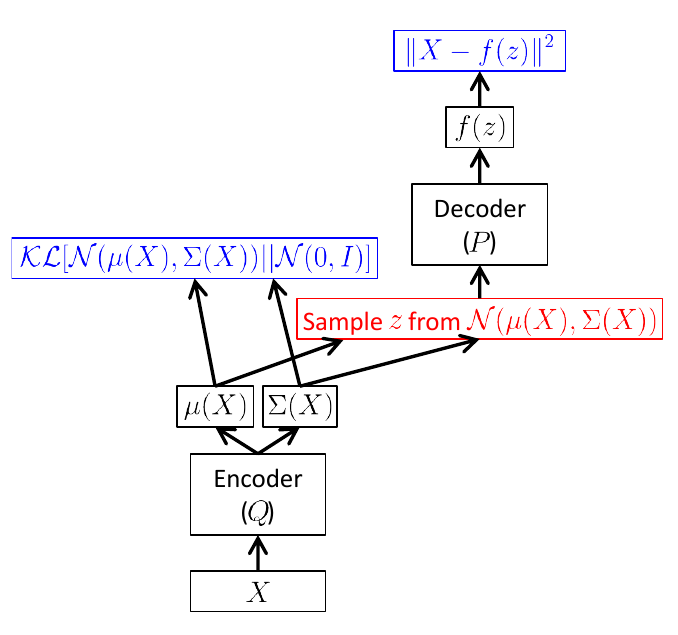
\includegraphics[height=6cm]{img/3_ML/VAE_tutorial_a.png} \label{fig:vae_tutorial_a}}
    \subfigure[]{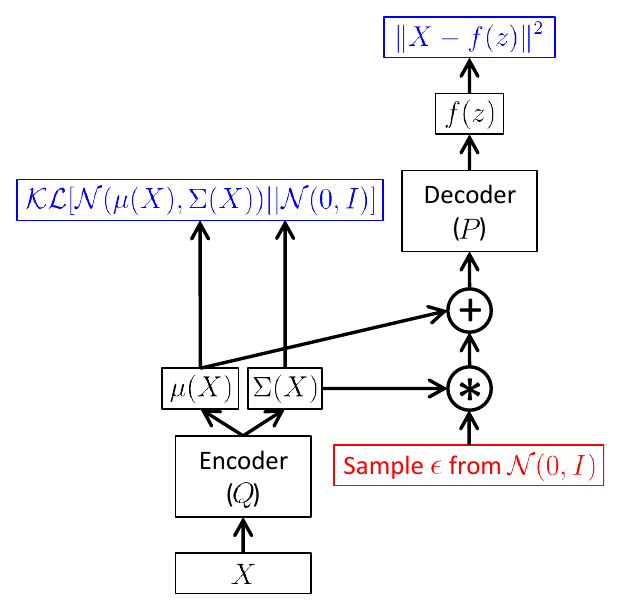
\includegraphics[height=6cm]{img/3_ML/VAE_tutorial_b.png} \label{fig:vae_tutorial_b}}
    \caption{Training representation of VAE (a) and the same with the applied "reparametrization trick" (b), where $p(x|z)$ is Gaussian. The red boxes shows sampling operations that are not differentiable, blue shows loss layers. Source:~\cite{doersch2016tutorial} }
    \label{fig:vae_tutorial}
\end{figure}
The neural network implementation is shown in \Figure{\ref{fig:vae_tutorial_a}}%(figura 4 sinistra) 
where the encoder computes $\mu(x)$ and $\Sigma(x)$ and the decoder computes $f(z)$. The terms in blue represent the loss function that has to be minimized over the parameters of the encoder and decoder. Still this schema has a problem: since a random sample gets sampled in the procedure, the overall function is not differentiable. However its structure is equivalent to \Figure{\ref{fig:vae_tutorial_b}} where sampling over $N(0,I)$ is performed at the sample selection.
This is called "reparametrization trick" and makes the overall function differentiable.



% We can now make a little digression on this result: the first term of the last equation is a likelihood expectation so it encourages densities that place their mass on latent variables that explain the observed data. The second term is the negative value of KL divergence between the variational density and the prior; so it encourages densities that are close to the prior. 
% Thus optimizing \acs{ELBO} means making the Bayes balance between likelihood and prior for the training dataset.
%
\begin{figure}
    \centering
    \subfigure{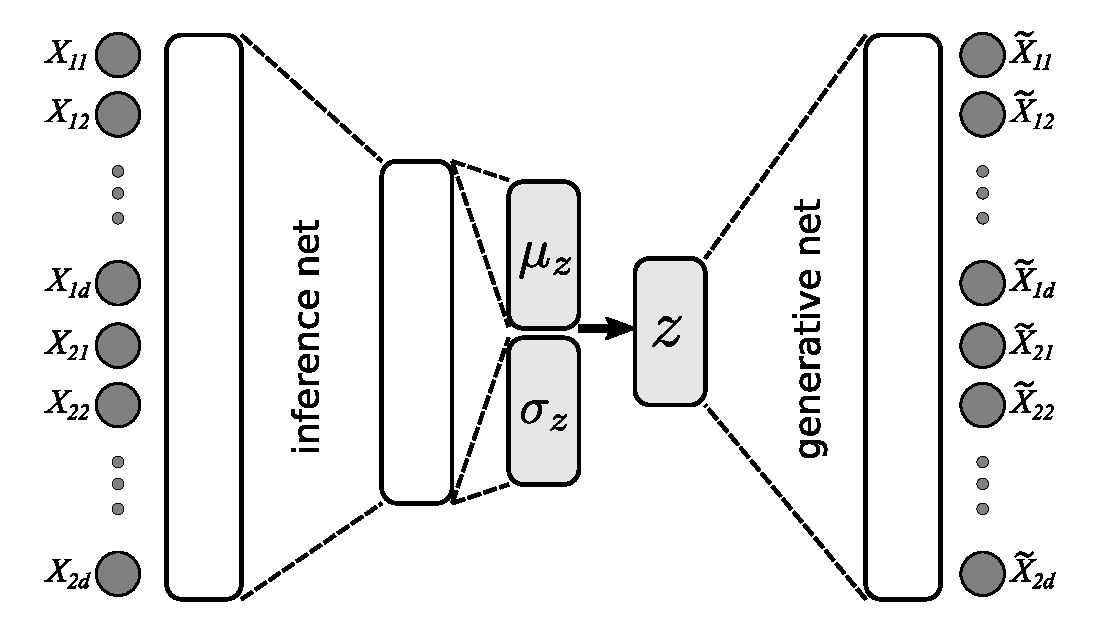
\includegraphics[height=4.5cm]{img/3_ML/VAE_1.pdf} \label{fig:step1_vae}}
    \subfigure{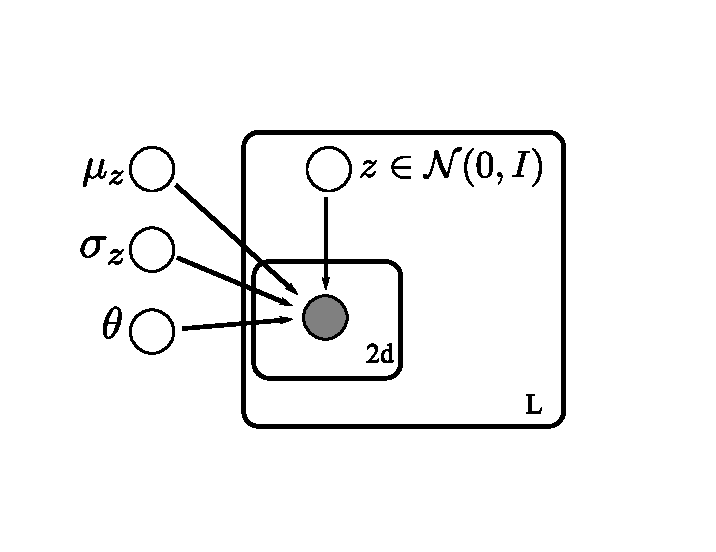
\includegraphics[height=4.5cm]{img/3_ML/VAE_1_plate.pdf} \label{fig:step1_vae_plate}}
    \caption{ The general description of a Variational Autoencoder shown both in its topological structure (left sketch), where the encoder and decoder are connected by inner reparametrization layers that form the inner latent space variables; and in \textit{plate notation} where all covariates are explained through latent variables (hidden "causes") with normal distribution. }
    \label{fig:step_1_VAE}
\end{figure}










%  _____ ___ _     _       _   _ _____ ____  _____ 
% |  ___|_ _| |   | |     | | | | ____|  _ \| ____|
% | |_   | || |   | |     | |_| |  _| | |_) |  _|  
% |  _|  | || |___| |___  |  _  | |___|  _ <| |___ 
% |_|   |___|_____|_____| |_| |_|_____|_| \_\_____|
%


\section{A simulated case study for latent space derivation}

To provide a good playground for the tests that we initially foresaw for this study, we built a simple algorithm to simulate possible dataset of one-dimensional signals. This may seem quite naive with respect to the complex \acs{DNN} inputs that characterize the latest works presented in this field, however it turns out to be worth for our purposes. Indeed it is very simple to manage, and it matches the simple case of the feature extraction applied to the acquisition device that we plan to add to experiment \acs{DAQ} system. Moreover it presents a quite widespread application in the area of signal conditioning all-over the experiment diagnostics: both in the temporal and in the spatial domain. For example the \acs{SXR} - that is our main case of study - provides as outputs a one-dimensional signal representing the spatial distribution of the electronic temperatures $T_e$ at time $t$. All data in this case are computed by measures of the integrated signal along the cords, and inverted to find the actual point temperature that is finally projected on the central axis in the equatorial plane crossing the center of the machine and the center of the chamber. The final output is a set of ordered points that can vary in: number (missing points for non working chords), position along projection axis, and temperature value.

\subsection{Gaussian sum generator}
\label{section: gaussian sum generator}
As a first very general approach we created an automatic generator of a one-dimensional sum of Gaussians envelopes. 
The generator is lead from a set of parameters, such as the number of points to generate, the random distribution of possibly missing values, the fixed missing positions, the added generation noise, and so forth. 
Once the generator is queried for a new instance, it selects randomly a label number that corresponds to a particular curve in a defined set of function classes. For the definition of gaussians we use a dictionary named \textit{kinds} that provides, for each possible label, a set of arrays in \textit{gain},  \textit{mean}, and \textit{sigma} for each of the sum of Gaussians components.
In \Figure{\ref{fig:sum_of_gaussians}} an example of five \textit{kinds} setup (also known as reconstruction labels) is shown with their respective representation curves. 
%
\begin{figure}
    \centering
    \begin{minipage}[b]{0.57\textwidth}
    \begin{lstlisting}[
        language=Python,
        basicstyle=\tiny,
        numbers=none,
    ]
 from Dummy_g1data import Dummy_g1data
 
 ds = Dummy_g1data( feature_dim=40, 
                    latent_dim=2, 
                    counts=10000 )
 ds.kinds = [
  {'gain': [1, 1],'mean': [0.2, 0.8], 'sigma': [0.1, 0.1]},
  {'gain': [0.5], 'mean': [0.8], 'sigma': [0.1]},
  {'gain': [0.5], 'mean': [0.2], 'sigma': [0.1]},
  {'gain': [1],   'mean': [0.5], 'sigma': [0.2]},
  {'gain': [0.5], 'mean': [0.5], 'sigma': [0.2]}
 ]
 ds.buffer() # buffer 10K samples in memory
 
 # adapt dataset generator to VAE with labels as input
 ds = ds.ds_array.map(lambda x,k: (x,x) )
 
 
    \end{lstlisting}
    \end{minipage}
    \hfill
    \begin{minipage}[b]{0.42\textwidth}
     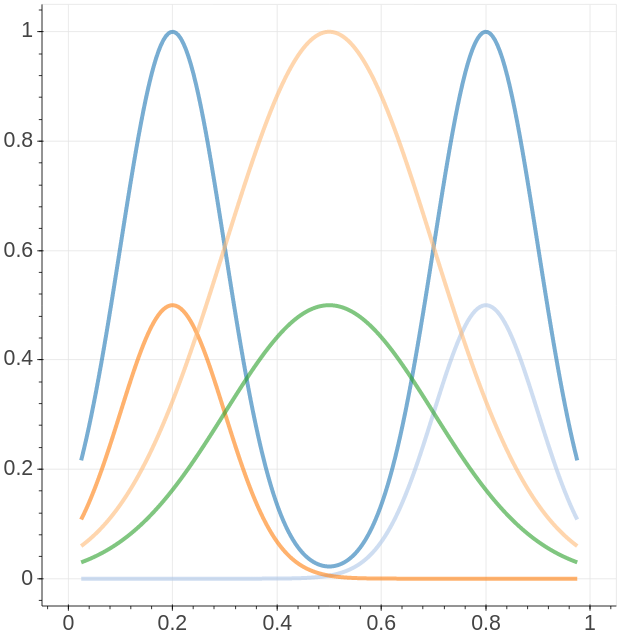
\includegraphics[height=5cm]{img/STEP1/dummy_kinds.png}
    \end{minipage}
    \caption{A generation setup example for five \textit{kinds} of sum of gaussians: on the left the dictionary that fills the parameters of the generator for each of the five classes; on the right a plot shows the five kind representations where colours helps to distinguish among them. }
    \label{fig:sum_of_gaussians}
\end{figure}
%
The generation of each dataset instance proceeds as described hereafter. At first we chose an ordered set of values along x-axis from a uniform distribution $\bm{x}_1 \in \mathbb{R}^{d}$ (with $x_{1,i} \geq x_{1,i-1}$), where $d$ is the number of desired points generated for each instance. Then, if not specifically asked, a label is also extracted from uniform random integers within the range of \textit{kinds} cardinality; and the related Gaussian exponential is applied for each of the parameter in that \textit{kind} and for each of the points. So a new set $\bm{x}_2 \in \mathbb{R}^d$ is created, in which:
\begin{equation}
    \bm{x}_2 = \sum_{k=1}^K \frac{1}{Z_k} \exp{-\frac{1}{2}\left( \frac{\bm{x}_1-\mu_k}{\sigma_k}\right)^2}
\end{equation}
The complete data sample we use as input will now be \textbf{any} combination of $\{\bm{x}_1, \bm{x}_2\}$; for simplicity we chose to construct data with the simple concatenation: $\bm{x} = [\bm{x}_1, \bm{x}_2]$ where now $\bm{x} \in \mathbb{R}^{2d}$.
The generator is configured as a tensorflow dataset that is directly fed into the autoencoder where we previously mapped \textit{data} and \textit{label} of each element both with $x$ values (we are not interested in label as VAE is an unsupervised method) to train \acs{VAE} with proper matching input and output.
A possible minimal configuration of data generator is shown in \Figure{\ref{fig:sum_of_gaussians}} where we have five classes of curves in the range $x_i \cap [0,1]$. The same set of curves are also plotted in dense domain to provide a ground-truth for plots. We chose to train a \acs{VAE} with only \textbf{two latent variables} (hereafter indicated as \VAE{2}), because the result is easier to represent by Cartesian axes. This actually limits the latent space representational power, but the issue will be discussed in a proper section.
%
\begin{figure}
    \centering
    \subfigure{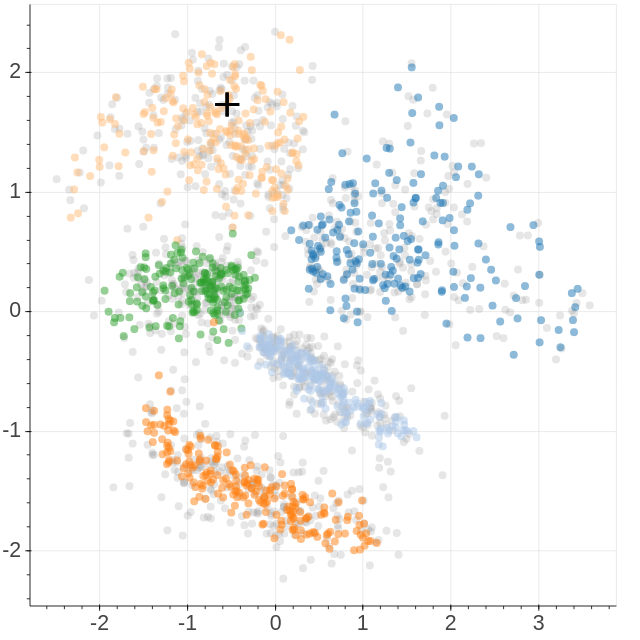
\includegraphics[height=4.5cm]{img/STEP1/ls1.png} \label{step1_1}}
    \subfigure{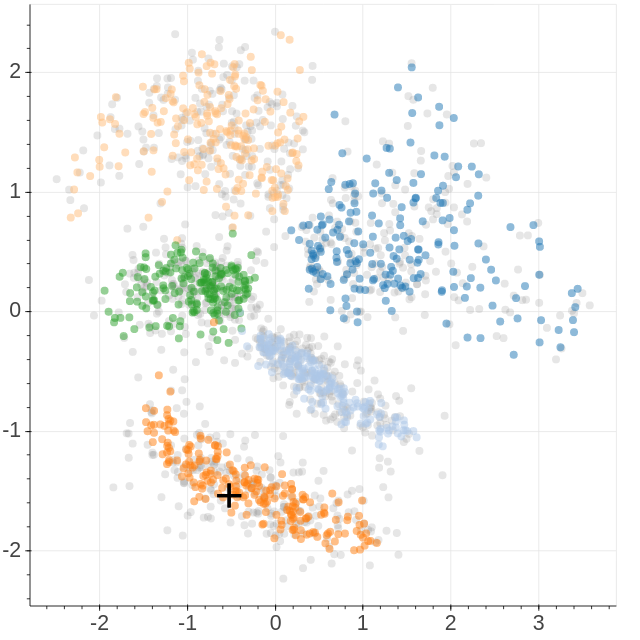
\includegraphics[height=4.5cm]{img/STEP1/ls2.png} \label{step1_2}}
    \subfigure{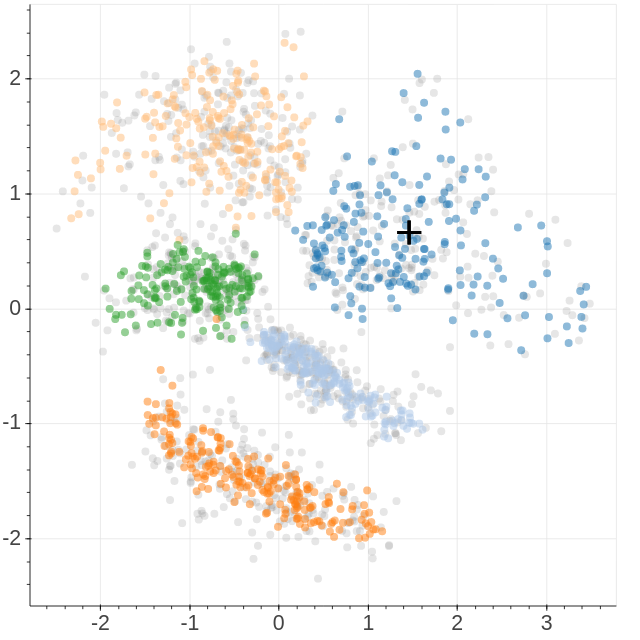
\includegraphics[height=4.5cm]{img/STEP1/ls3.png} \label{step1_3}}
    \subfigure{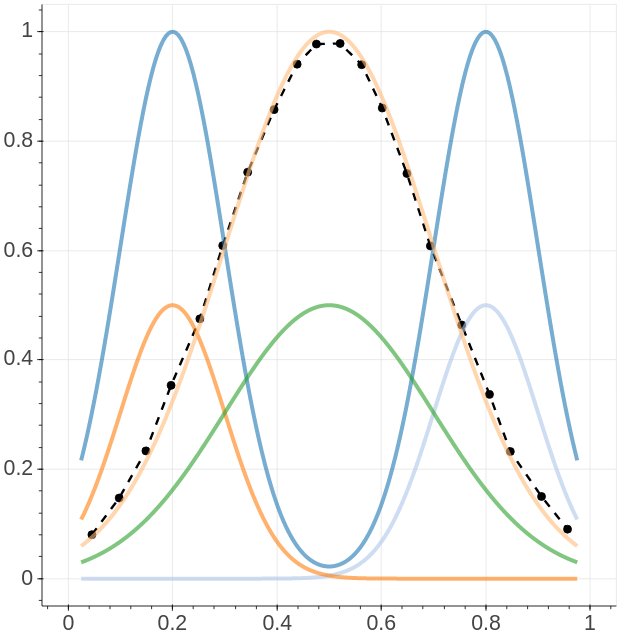
\includegraphics[height=4.5cm]{img/STEP1/gn1.png} \label{step1_4}}
    \subfigure{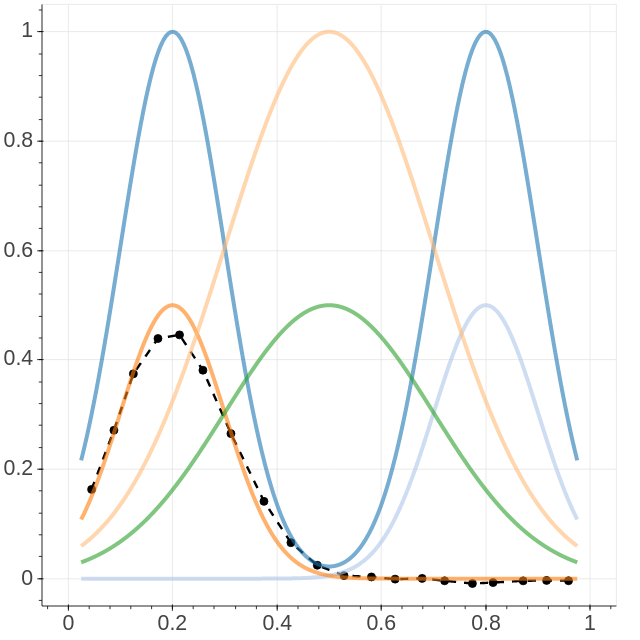
\includegraphics[height=4.5cm]{img/STEP1/gn2.png} \label{step1_5}}
    \subfigure{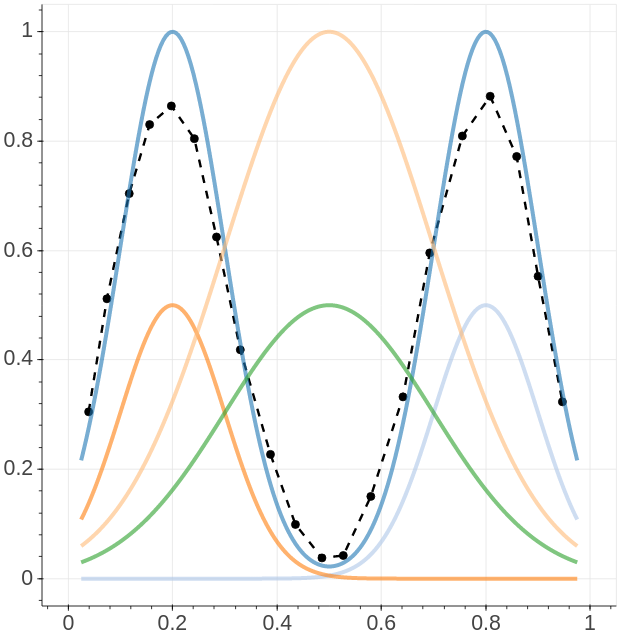
\includegraphics[height=4.5cm]{img/STEP1/gn3.png} \label{step1_6}}
    \caption{ Three instances of latent space reconstruction from \VAE{2} starting from a latent position indicated with ($\bm{+}$) in the scatter plot on top that corresponds to the black curve from decoder output plotted on bottom. In the upper figures the scatter plot shows also 1000 samples from validation dataset where the colour position indicates the encoded mean $\bm{\mu}_z$ and the corresponding class in the colour scale, while the grey plot is a reconstruction of the $\bm{\sigma}_z$. The clusters color is also matching the corresponding \textit{kind} of curve that is plotted for reference on bottom figures.} 
    \label{fig:step_1}
\end{figure}
%
In \Figure{\ref{fig:step_1}} three examples of \acs{VAE} reconstruction have been plotted. The parameters for the generator were $d=20$, no generation noise have been applied and the latent space is 2-dimensional. Latent space variables $\bm{z}$ are characterized by their variational parameters, i.e. $\bm{\mu}_z$ and $\bm{\sigma}_z$, and those parameters are plotted in the same figure for the three examples in the top set of graphs for 1K samples of the validation dataset. The scatter plot shows a coloured dot corresponding to the inferred latent position in \textit{xy-axis} and the respective \textit{kind} on the colour scale. A further grey dot is also plotted for each of the latent samples after the variational has been applied to generate a Monte Carlo approximation of the training process $\mathcal{N}(\bm{\mu}_z, \bm{\sigma^2}_z)$.
The same figure shows also an instance of the generative network output with black dots in the lower plots that have been overimposed to the ground-truth curves \textit{kinds} to see the matching. The reconstruction corresponds to the black cross ($\bm{+}$) in the latent space. It is worth to highlight the fact that this ($\bm{+}$) point was a generated point in the latent space and does not correspond to any sample of either the training set or the validation set. It is a new \textit{unseen} generation instance that lies within the latent space in the corresponding class cluster, but from the trained generator point of view, there are actually no more correlations with the input data. This also corresponds to the Bayes idea where the generated instances are only related to the latent "cause", once we fixed the trained parameters (see plate notation in \Figure{\ref{fig:step1_vae_plate}}).
Those plot have been generated using the utility functions we implemented for \RFXhunch exploiting the \textit{Bokeh}~\cite{bokeh} library for python and JavaScript. This can provide a useful scope to see the behavior of the decoder moving interactively the point in the 2D latent space, and looking at the reconstruction on the generated plot.
The complete \RFXhunch package will be described with more detail in \cref{section:RFXhunch}.
%
\subsection{Generative morphing effect}
When we play with joint encoder/decoder networks, that are our tools to step in and out of the latent space, \acs{VAE} is thought as a directed \acs{RBM}, and it is claimed to extract a meaning from data by extracting latent "concepts" and expanding them to the feature space. On the other hand, we have already pointed out that the generative effect of \acs{VAE} is also that, once trained, it maintains no actual relation with the data and can generate samples by only means of decoding the latent space. This becomes clear if we sample a point that is far from the dataset encoded clusters; for example, in \Figure{\ref{fig:step1_morph}} two latent space points ($\bm{z}_1$ and $\bm{z}_2$) have been reconstructed by generative network. 
%
\begin{figure}
    \centering
    \subfigure{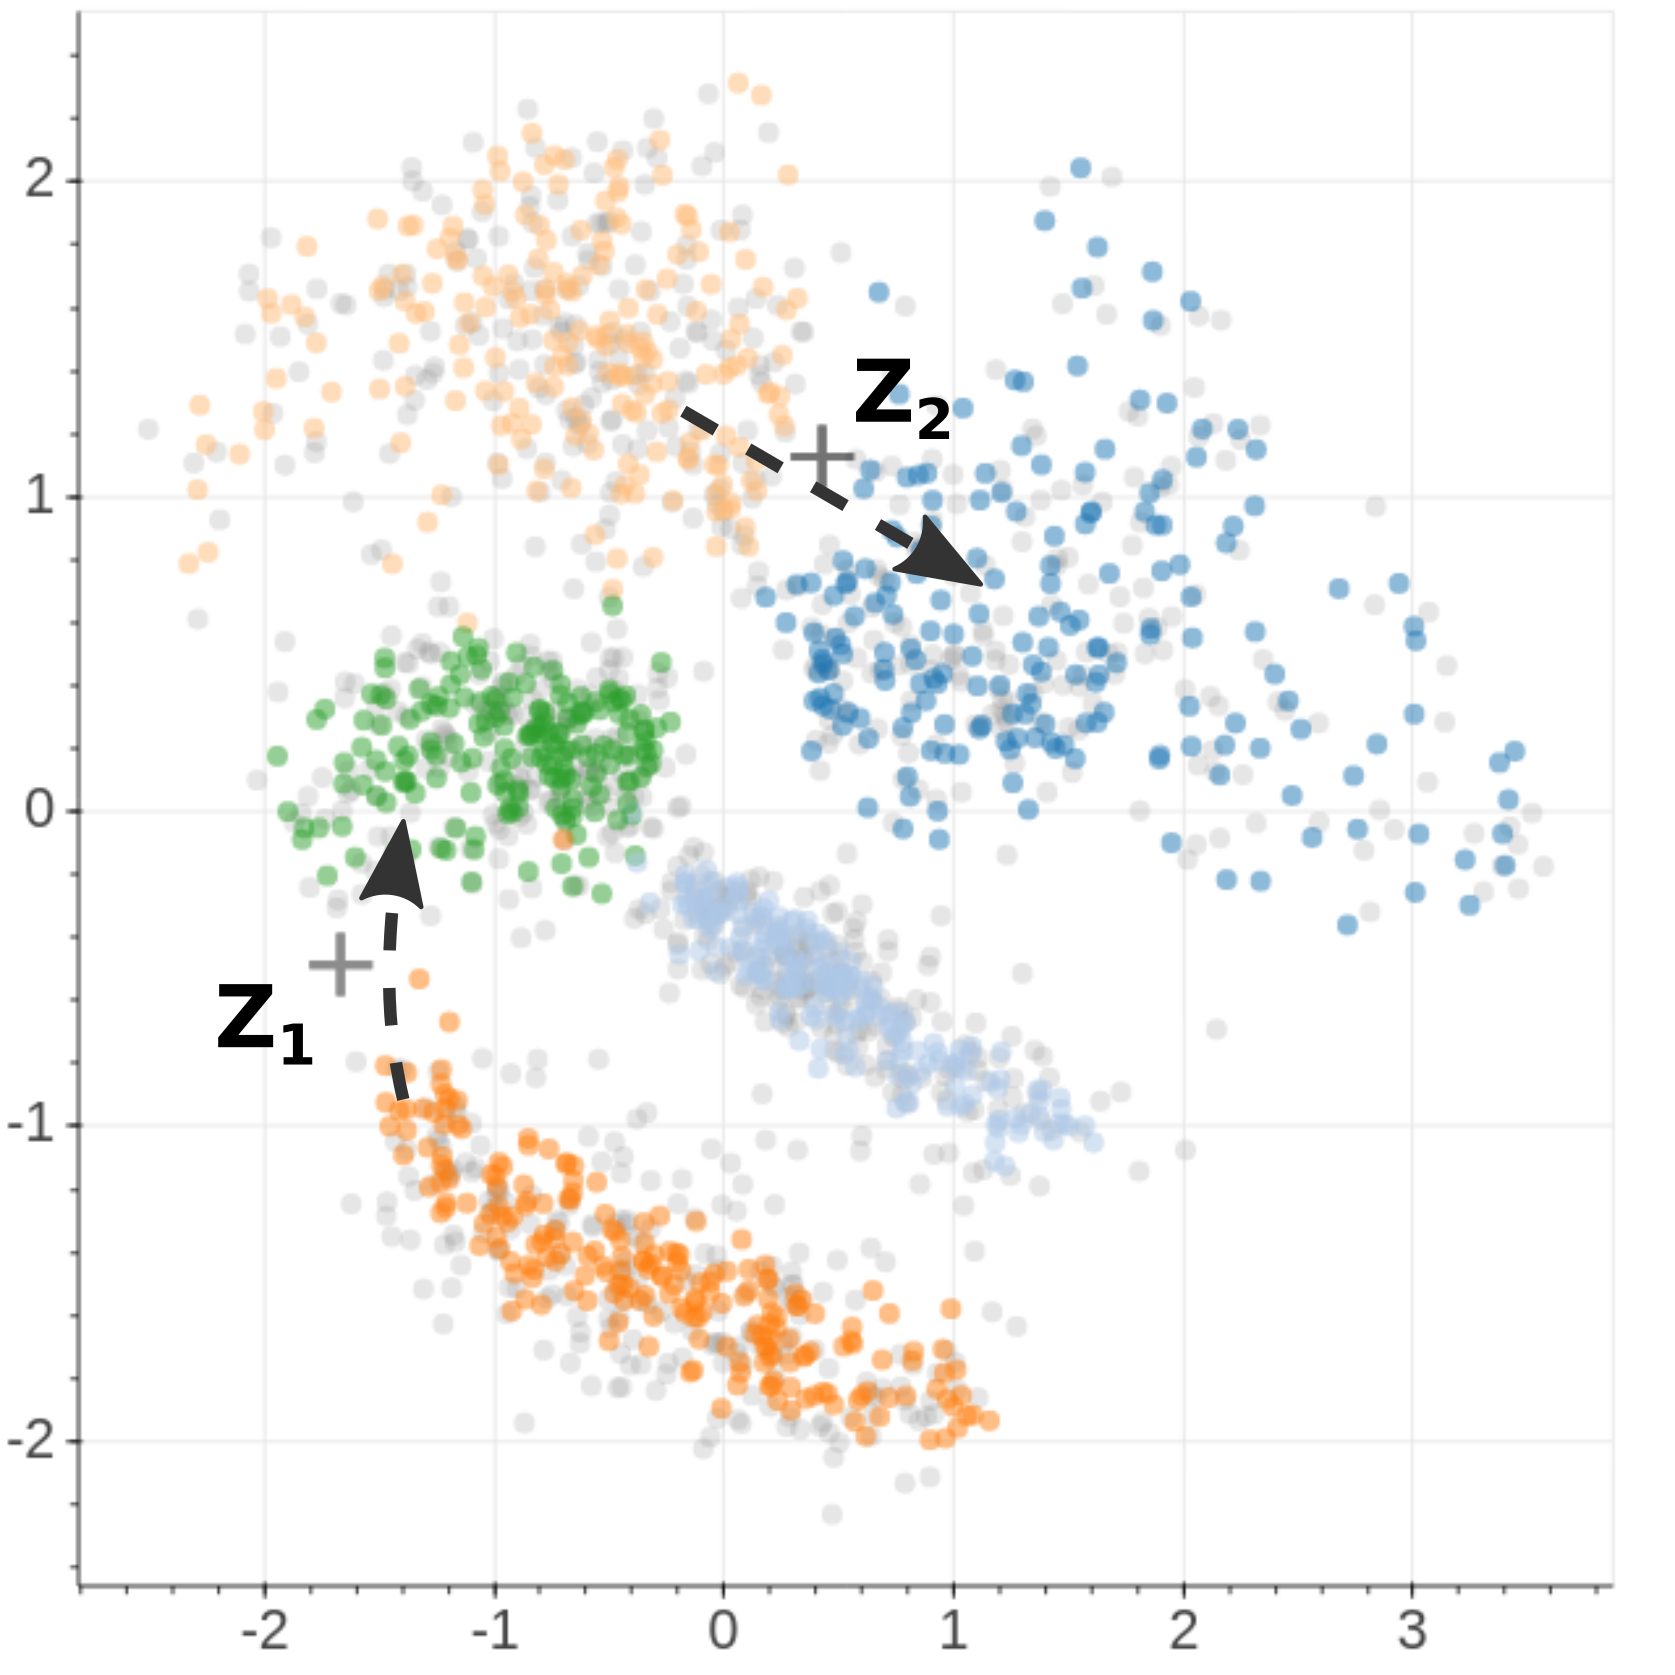
\includegraphics[height=4.5cm]{img/STEP1/morph_Z1Z2.png}\label{fig:step1_morph_z1z2}}
    \subfigure{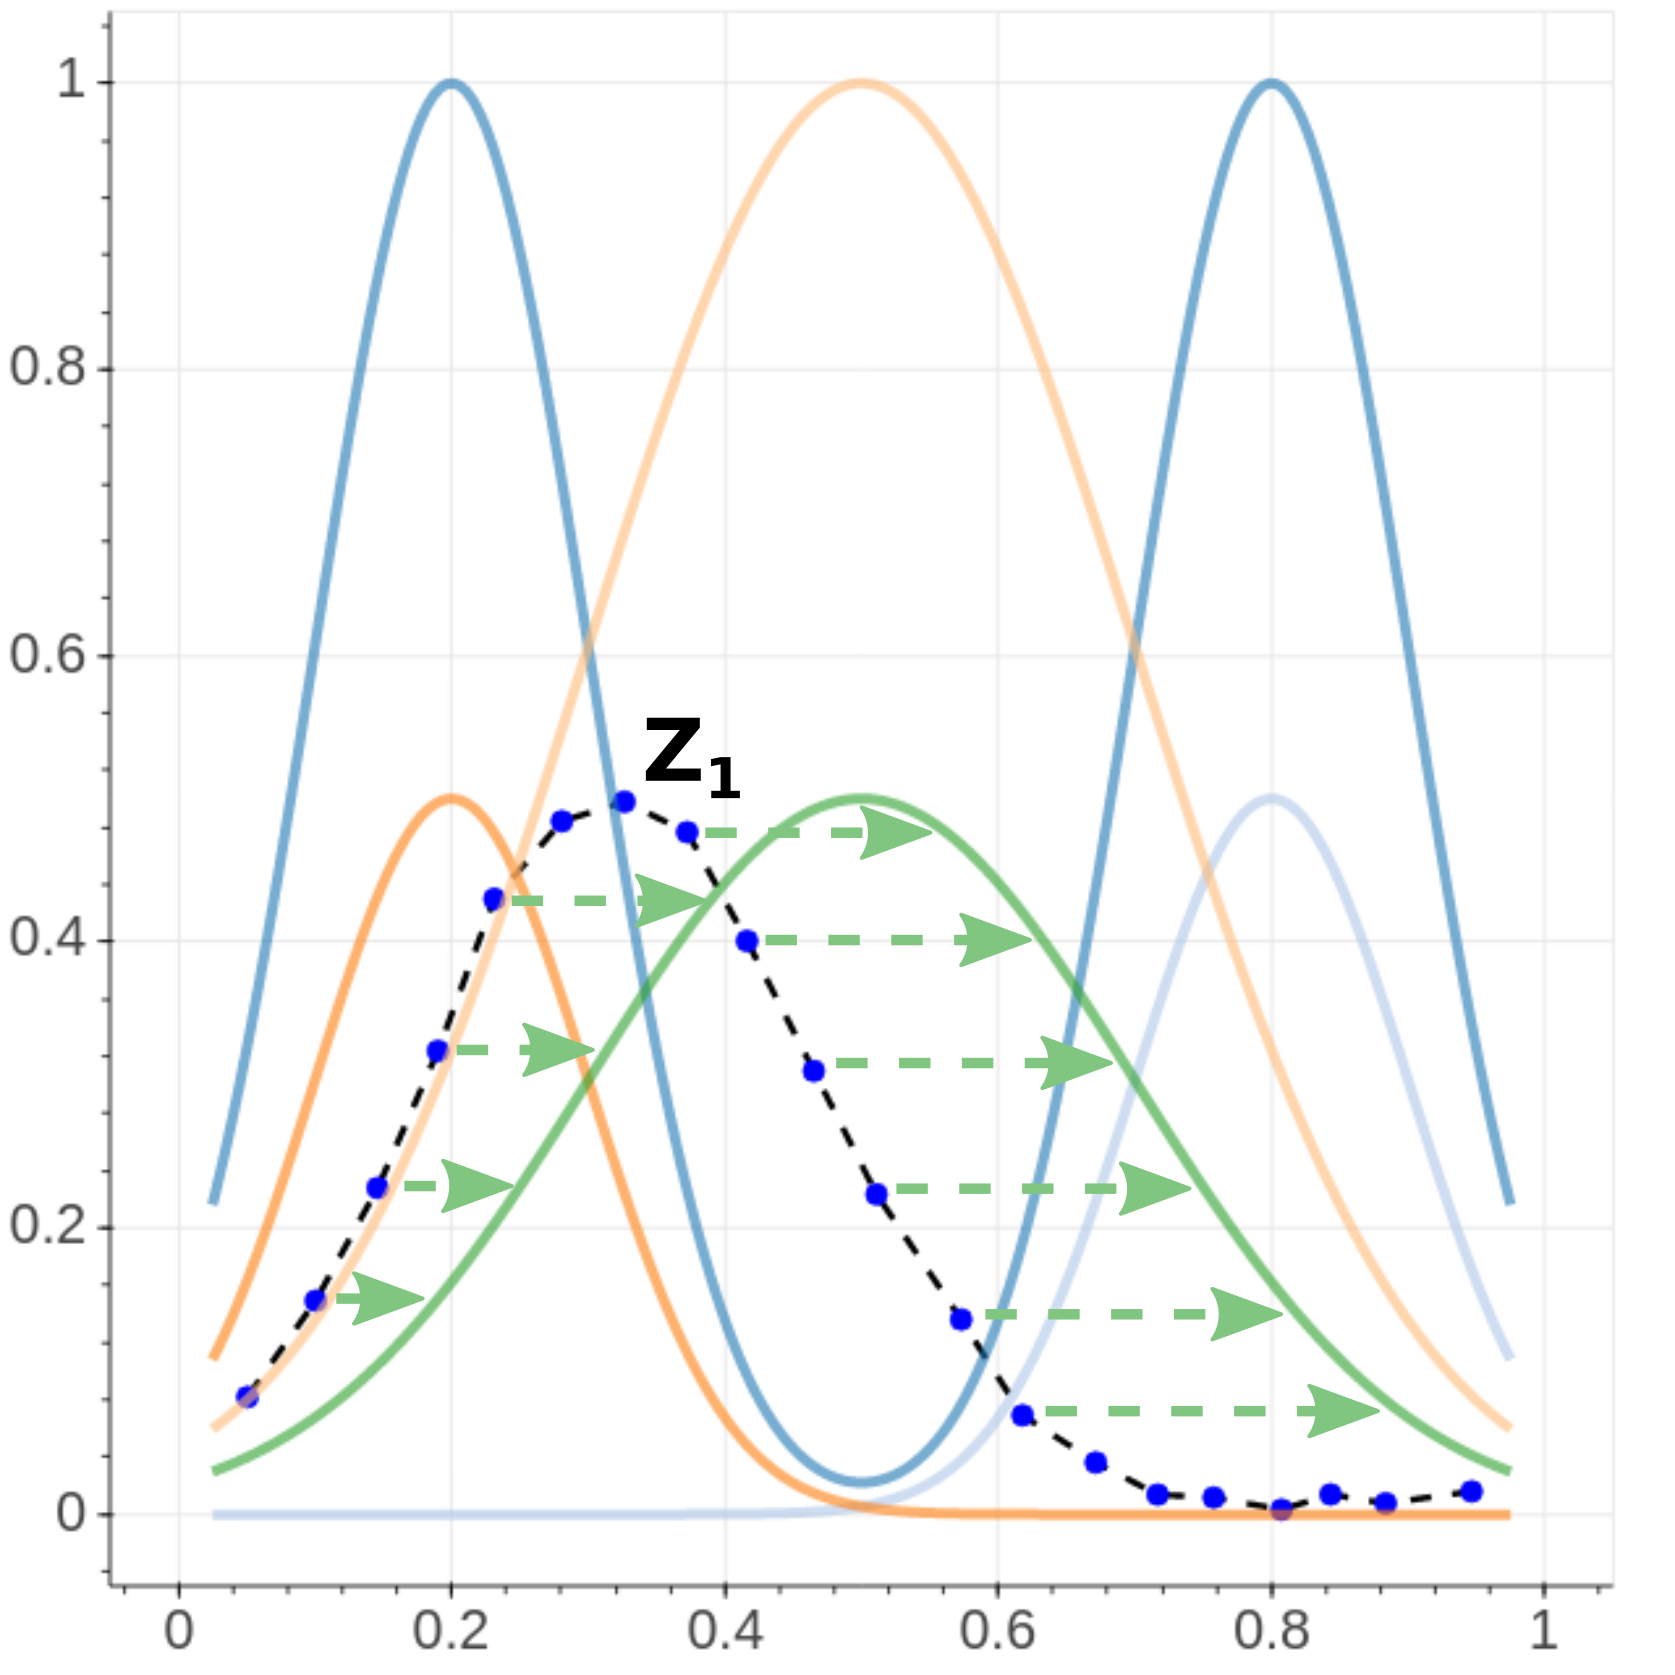
\includegraphics[height=4.5cm]{img/STEP1/morph_gn2.png} \label{fig:step1_morph_gn2}}
    \subfigure{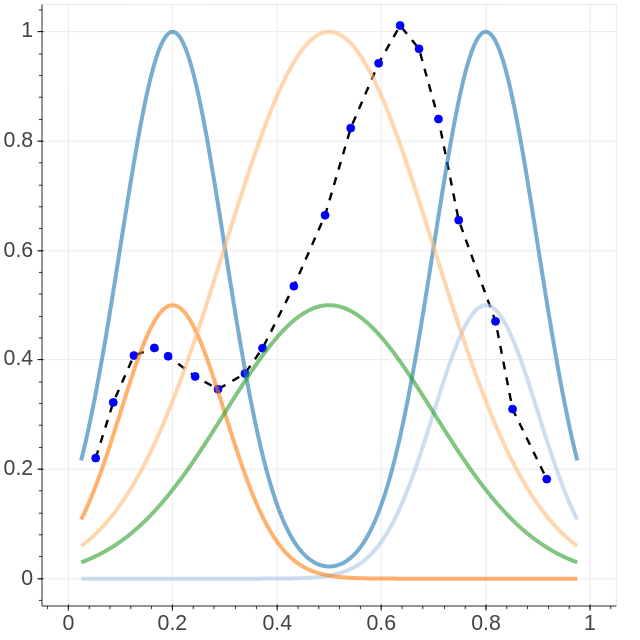
\includegraphics[height=4.5cm]{img/STEP1/morph_gn4.png} \label{fig:step1_morph_gn4}}
    \caption{Generative morph effect on reconstruction from \VAE{2}: two latent space points taken from middle space between clusters has been decoded and show how the generative effect can create solutions for non existent data "morphing" one class to another. } 
    \label{fig:step1_morph}
\end{figure}
It is quite clear from these figures the real power of the latent space: if we paint the reconstructed signal from all points in the latent space, we just traversed all possible configuration that the outputs can assume, so once we know how this space is shaped we can lead the output to maintain certain characteristics. For instance, we can constrain the system to remain within some predefined boundaries thus implementing a very simple, but robust, non linear control on the outputs.

\subsection{Latent space topology}
%With the description of \textit{linear factor analysis} in \cref{linear factor analysis} the unidentifiability of the latent variables has been introduced; so unfortunately upon each training the latent space assumes a different configuration. 
Beside the simple generation on points that lies in the latent "\textit{interstitial}", it can be argued which possible configurations the latent space itself could assume. Given the fact that the purpose of \acs{VAE} is to adapt the space upon jumps between clusters of similar features, the idea is that we could imagine to simplify the entire cluster with its center of mass, and separate the space itself in corresponding regions. This could be easily done with the unsupervised k-means algorithm with k corresponding to the k classes ( the \textit{kinds} ) letting it find the means for each center of mass. At this point we could have an algorithm that actively classifies the features upon latent representation, while in the latent space this classification can be plotted by the classical \textit{Voronoi diagram} as shown in \Figure{\ref{fig:voronoi_ls}}. With these defined regions we can say that a curve is of a certain class if its latent coordinates are within the corresponding region $k_i$; but what happens in the boundaries? In the previous section it has been shown that the algorithm tends to make a morphing adjustment to the signal shape to make the step from one region to the other as smooth as possible, however it is not always a feasible solution. For instance, as it can be seen in \Figure{\ref{fig:step1_morph_gn4}}, passing from the central Gaussian curve to the double one requires a steep movement on the position of generated points.
Although the topological configuration of the latent space remains generally unidentifiable, and so does the clusters organization, looking back carefully at \Figure{\ref{fig:step_1}} an overall structure among the samples placed by the encoder in the scatter plot can be glimpsed. For example, the two single Gaussian curves that have been defined at plot center (i.e. the curve generated from the last two \textit{kinds}: $k_4, k_5$), corresponding respectively to the $\bm{A}$ cluster (green) and the $\bm{B}$ cluster (top light-orange) have been placed close to each other. And this configuration repeats with high probability with different trainings; this happens because the algorithm finds "easy" to generate a transition from these two classes, that is the total amount of point movements remained small for each of the training attempt. The same happens for the tree curves at the lower part of the plot: the left orange (\textbf{E}), the previous central green one (\textbf{A}), and the azure one (\textbf{D}). In addition, the shift transition of the Gaussian points protrusion from left to right is actually a "C" shape curve in latent space, because the algorithm chose to guarantee the transition from $\bm{D}$ to $\bm{E}$ as well. That is because the total cost (meant as the integral of the computed loss) associated with that transition (i.e. the rise of the bent on one side and the fall of the bent in the other) is also small with respect to other transitions. On the contrary a complete symmetry should exist between the transition from curve \textbf{D} to \textbf{C} and from curve \textbf{E} to \textbf{C}, so those groups of samples could be thought to be equally close to each other; but the training decided for one or the other arrangement, because it is associated to a steeper change on reconstructed points than the other solutions. A natural parallelism of such cost transition with the field theory could be argued and indeed a perturbation approach to the study of latent space structure has been recently proposed in~\cite{andrsterr2019perturbation}. Associating an energy jump upon classes helps to identify which are the main degrees of freedoms for the latent variables in performing transitions or any movement in the latent space (remember that we are not bounded to the simple case of multi-class classification).
In \Figure{\ref{fig:voronoi_2d}} a connected graph has been drawn to plot all possible transitions among classes of the reported example, that is actually the dual representation of the Voronoi diagram of \Figure{\ref{fig:voronoi_ls}}. Imaging each edge as the minimum energy path to cross the boundary between two classes, the number of possible free edges would be strictly linked with the latent space dimensionality: for 1-dimensional latent space 3 classes can be represented, 4 classes can be represented with a 2-dimensional space and 5 classes with a 3-dimensional space, and so forth. 
The idea behind this is the possibility to draw a graph with no crossing edges to create a smooth transition with any possible couple of knots in the graph. However because the actual crossing edges between clusters can be associated with the energy of the system configuration, there can be some solutions where the same configuration can explain many edges; an example is provided by the proposed set of classes where transitions $\bm{A} \rightarrow \bm{C}$, and $\bm{B} \rightarrow \bm{D}$ are matching with a unique representation in a crossing point. 
Conversely, the only way for $\bm{E}$ to reach $\bm{C}$ would be to spread around either $\bm{D}$ or $\bm{A}\cup\bm{B}$ with a sensible loss of energy for the cluster that would fade out the description of the $k_3$ covariates, thus being unfeasible for the optimum representation reached by the \acs{VAE}.
In any case the distance between $\bm{E}$ and the other clusters represents a limit on the overall optimization, and a possible way around this limitation is to increase the dimensionality of latent space (i.e. the number if the embedding neurons) as proposed in~\Figure{\ref{fig:voronoi_3d}}.
\begin{figure}
    \centering
    \subfigure{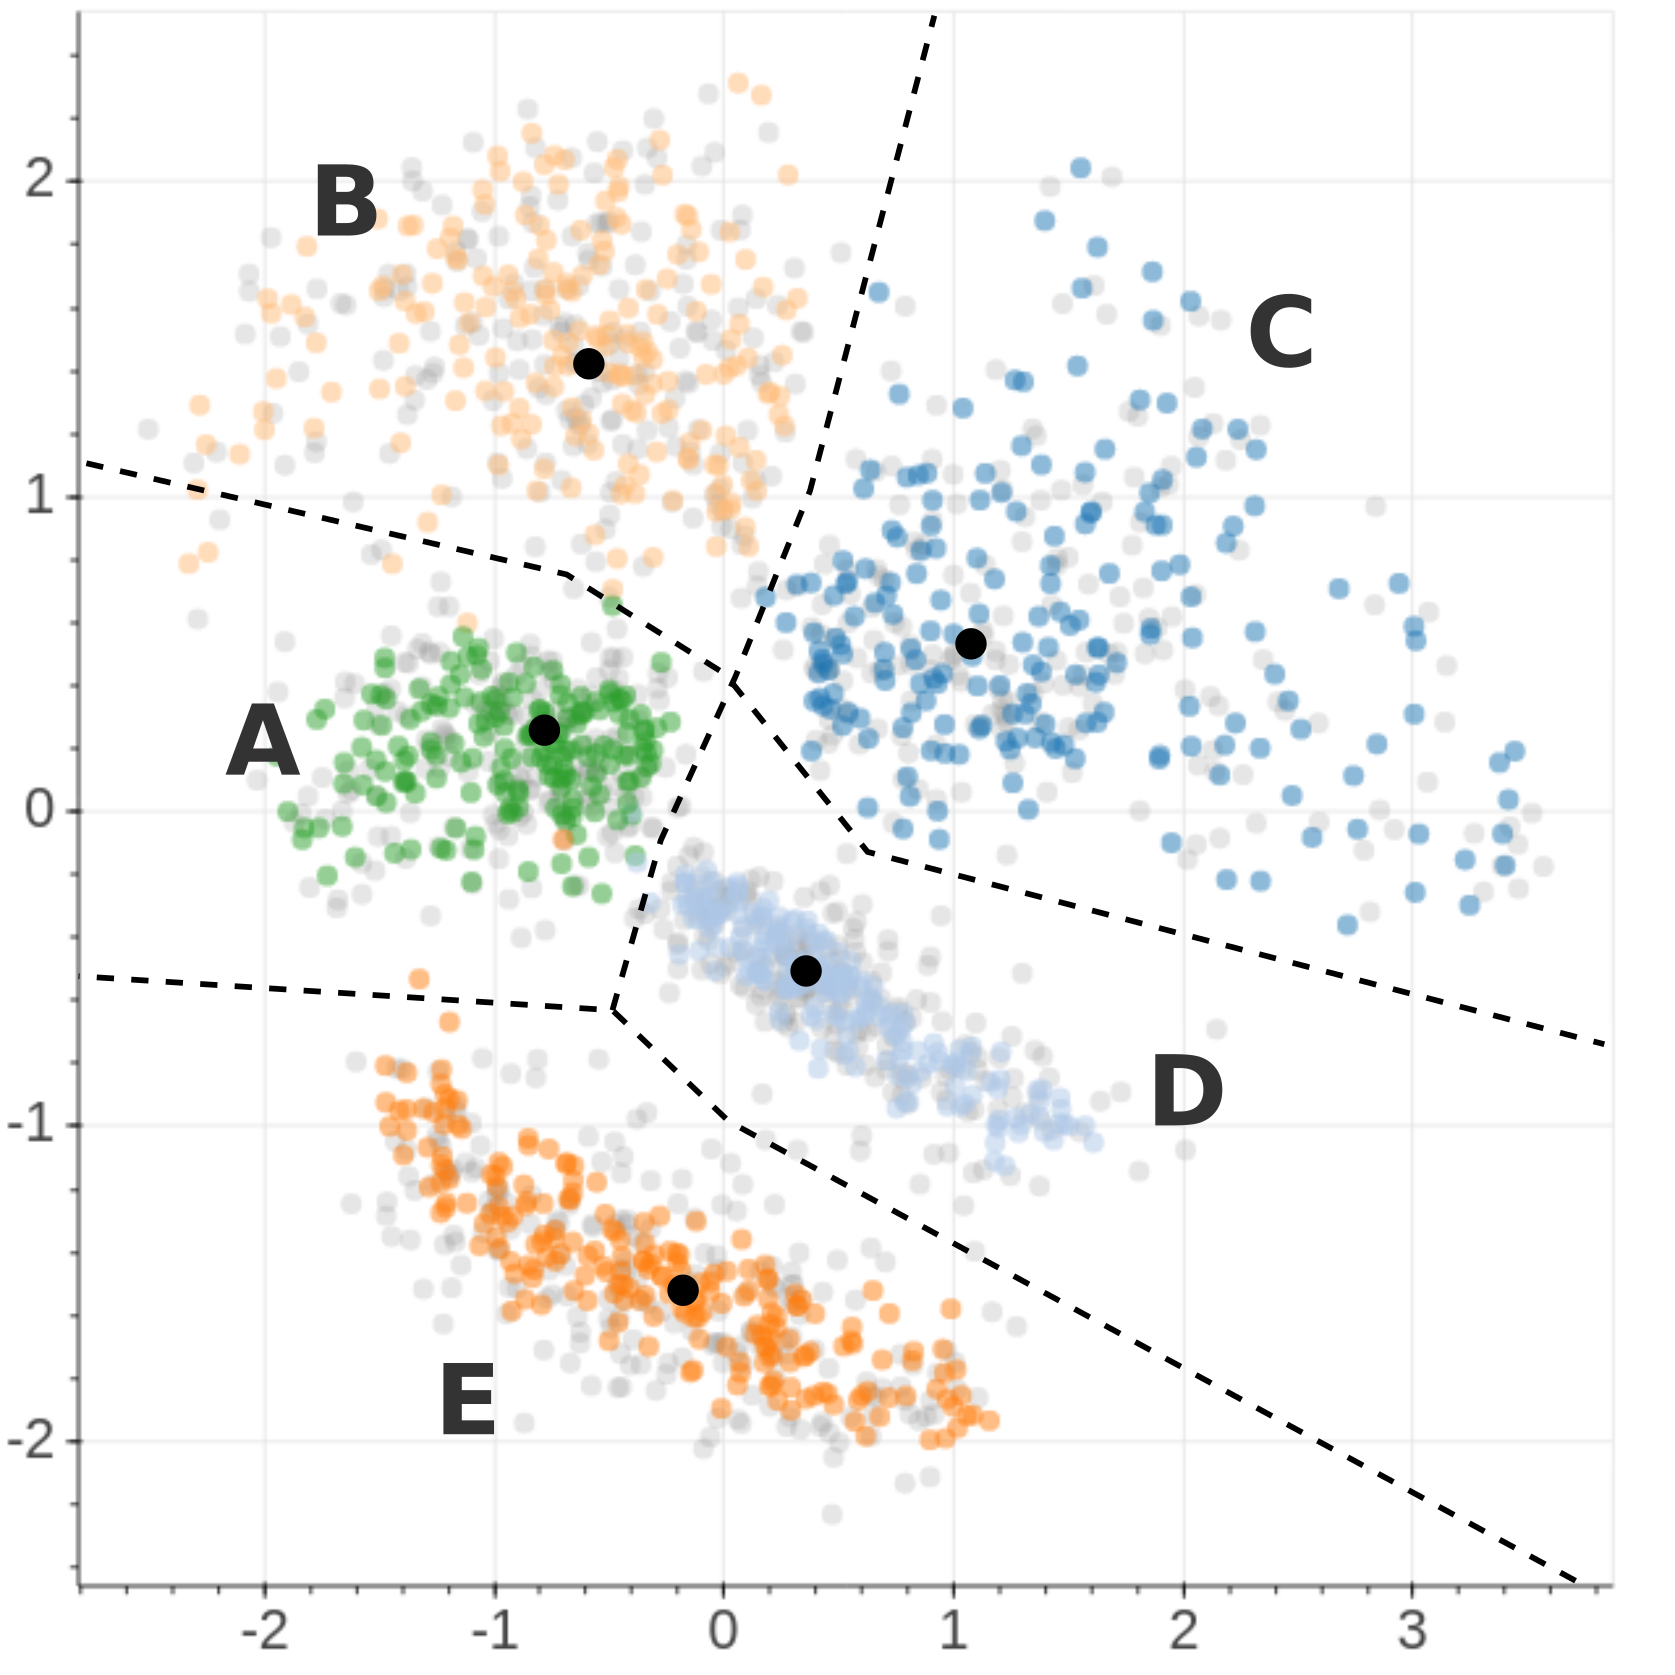
\includegraphics[height=4.5cm]{img/STEP1/voronoi_ls.png}\label{fig:voronoi_ls}}
    \subfigure{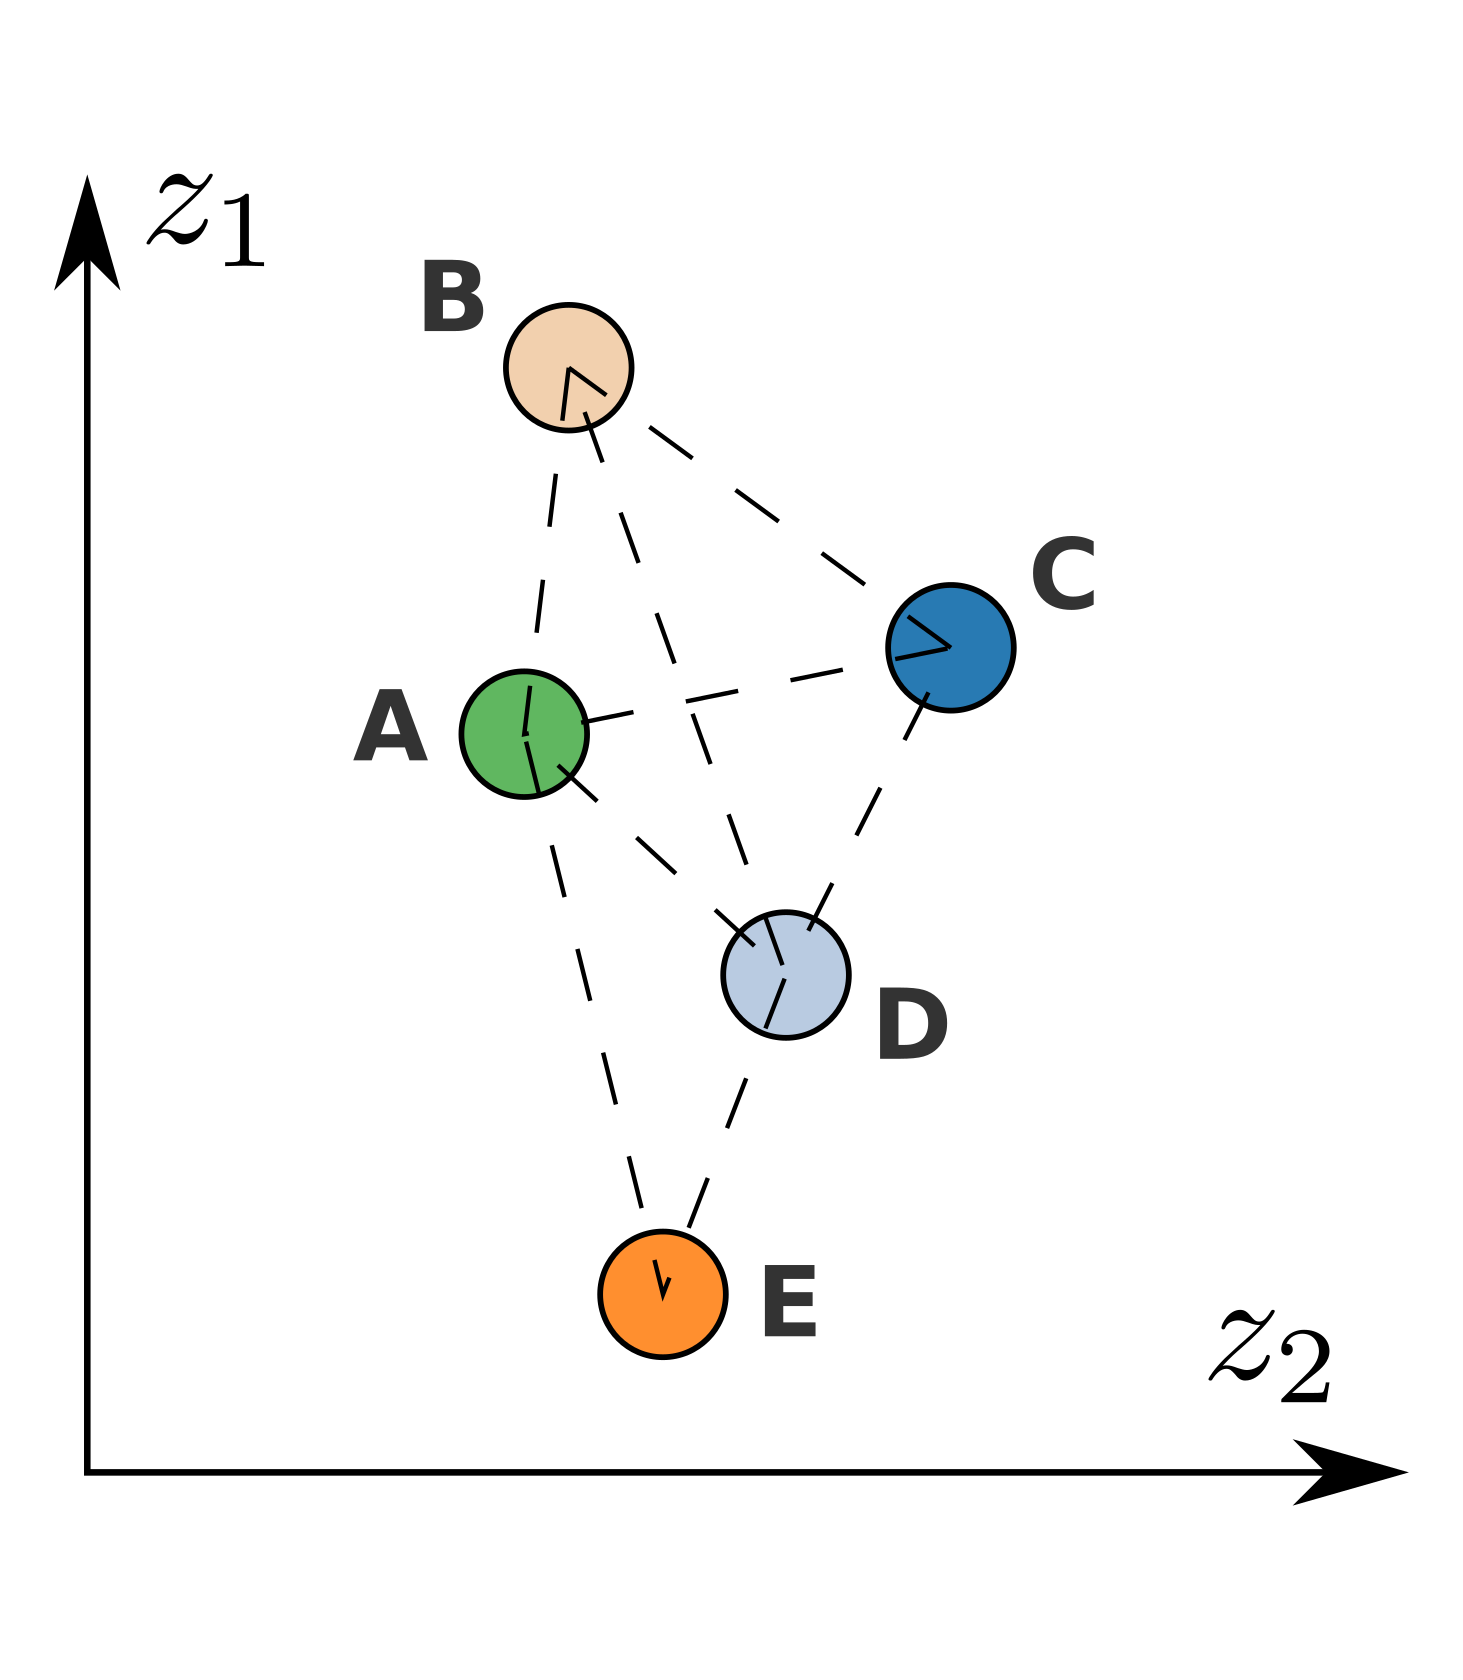
\includegraphics[height=4.5cm]{img/STEP1/voronoi_sketch_2d.png} \label{fig:voronoi_2d}}
    \subfigure{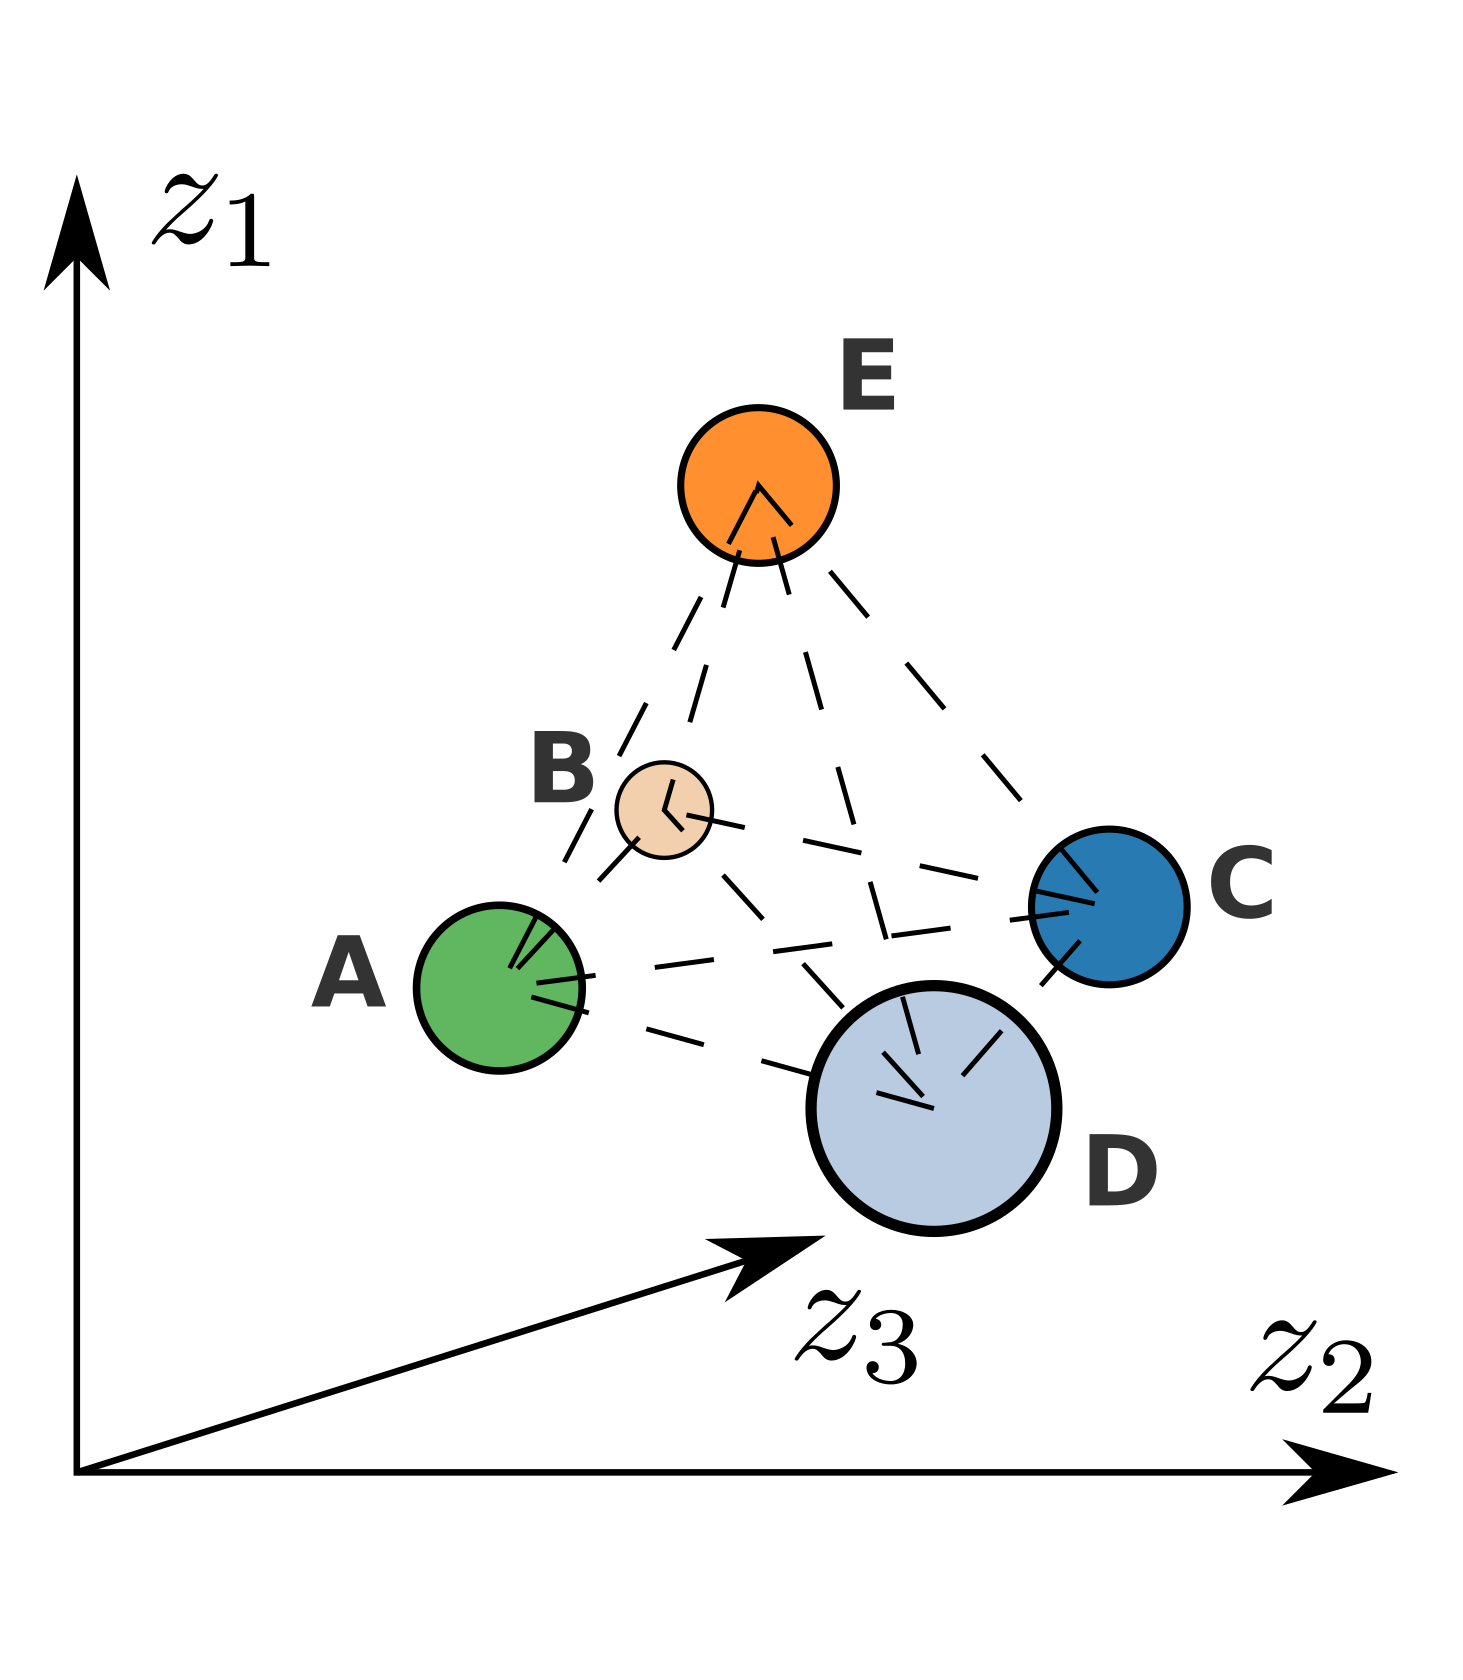
\includegraphics[height=4.5cm]{img/STEP1/voronoi_sketch_3d.png} \label{fig:voronoi_3d}}
    \caption{Topology configurations that are automatically generated upon the training of autoencoder } 
    \label{fig:voronoi}
\end{figure}

\subsection{Elastic fitting}
Even if the representation of \VAE{2} seems to present limitations on some class transitions, it is although providing a good fitting for the classes in the proposed example as already shown for three instances in~\Figure{\ref{fig:step_1}}. But what has not been shown yet is that there actually is a further subtle structure of the input dataset generator that \VAE{2} captured from the covariates. It is another implicit degree of freedom that comes from the fact that we chose to sample along the x-axis from a \textbf{uniform ordered} distribution; this generates samples that are free to span all along the axis, but chained with the strict inequality: $\{\bm{x} | x_{i} \geqslant x_{i-1}\}$.
\begin{figure}
    \centering
    \subfigure{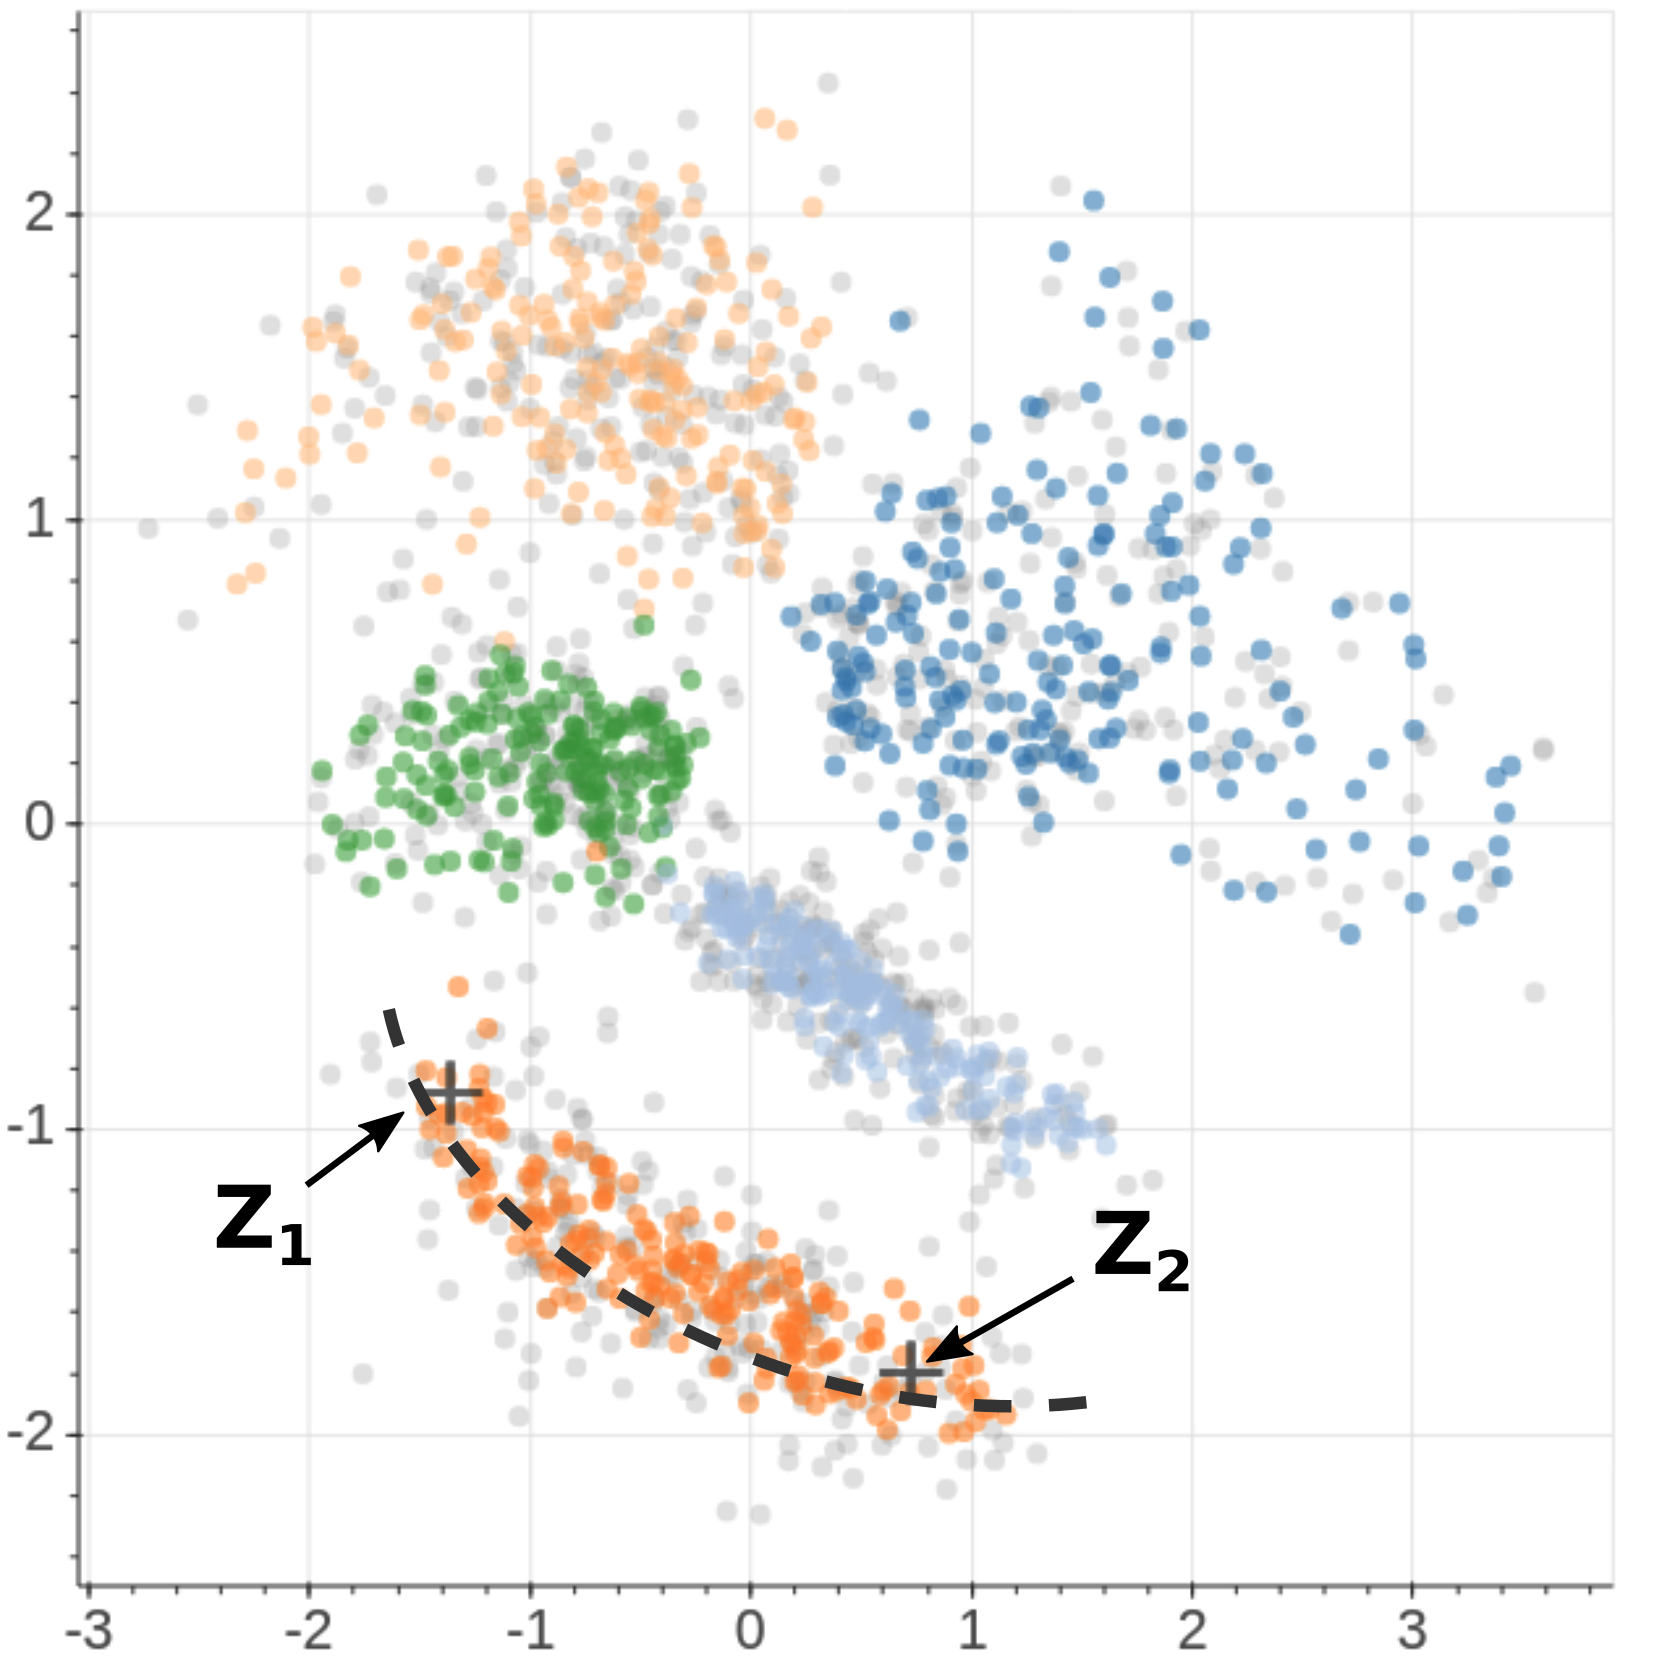
\includegraphics[height=4.5cm]{img/STEP1/elastic_Z1Z2.png} \label{fig:step1_elastic_z1z2}}
    \subfigure{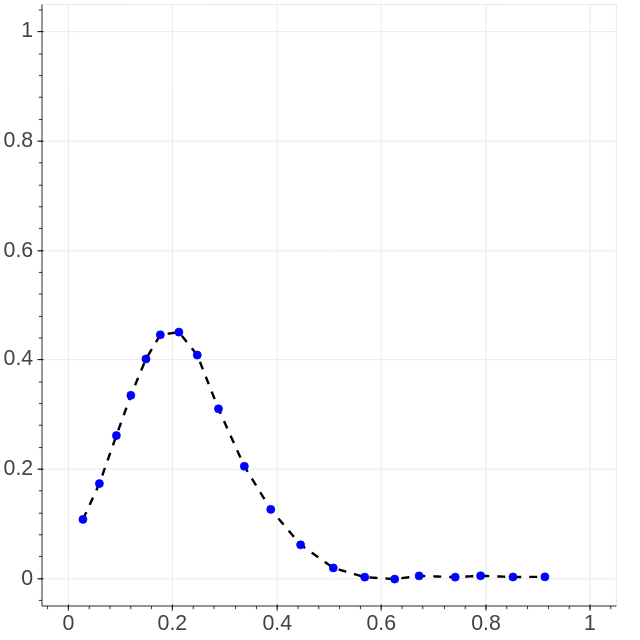
\includegraphics[height=4.5cm]{img/STEP1/elastic_gn1.png}  \label{fig:step1_elastic_gn1}}
    \subfigure{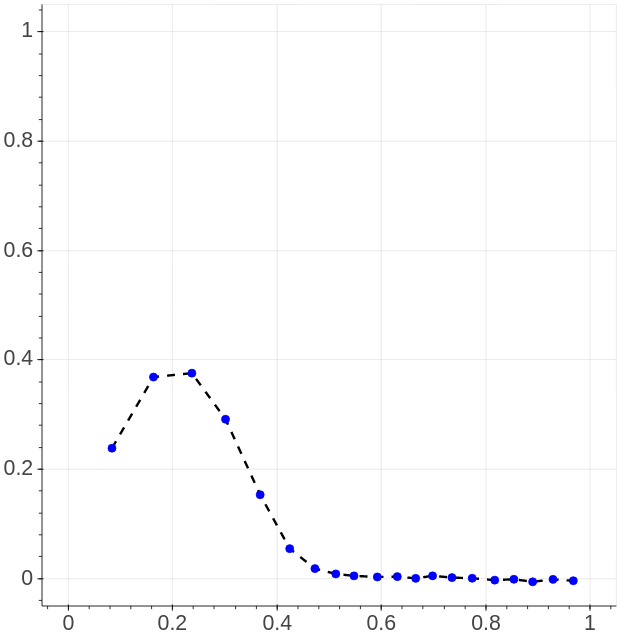
\includegraphics[height=4.5cm]{img/STEP1/elastic_gn2.png}  \label{fig:step1_elastic_gn2}}
    \caption{Elastic latent space reconstruction from \VAE{2} with scatter plot of the latent space and two samples of the same decoded class, where it can be seen that the autoencoder distributes the $\bm{x}_1$ positions degree of freedom of the database along the dashed line. Two samples $\bm{z}_1$ and $\bm{z}_2$ have been also plotted from the decoder output to see the elastic effect of the curve points distribution. } 
    \label{fig:step1_elastic}
\end{figure}
This further subdivision of the latent space is hidden in the shape of clusters themselves within one elongated direction. A clear example is visible in~\Figure{\ref{fig:step1_elastic}} where two latent variables points have been decoded and plotted in~\Figure{\ref{fig:step1_elastic_gn1}\ref{fig:step1_elastic_gn2}}; the effect of the x-axis dispersion fit is shown by the fact that even if the overall reconstruction of the curve is quite similar for all chosen points, the density of points is different along the axis. Moving one way or the other along the cluster generates curves that remain almost steady in y-axis but wobble in the x-axis density elastically adapting at best all possible choices of points that represent the generating Gaussian formula.

\section{Latent space regularization and disentangled representation}
In the previous section~\cref{section:training_regularization} the concept of \textit{regularization} has been introduced for a supervised network training; in this section some further methods will be discussed, applied to the \acs{VAE} and the latent space reconstruction.
%
One of the major challenges for today machine learning approaches is the fact that the resulting learned task can vary significantly depending on the choice of the data representation, i.e. the structure of the latent space.
It has been suggested that learning a disentangled representation of the generative factors within covariates can be useful for a large variety of tasks and domains~\cite{Bengio_2013}~\cite{ridgeway2016survey}. A complete disentangled representation can be defined as the network configuration where a single latent unit is sensitive to changes in a single generative factor, while being almost uncorrelated with all the others.
For example, a model that implements a deep convolutional \acs{VAE} trained on a dataset of objects images might learn independent latent units that are sensitive to data generative factors, such as the actual object class, the position, scale, or colour; thus each latent variable acts as a single self sufficient inversion model. And the most important outcome is that in a disentangled representation, knowledge about one factor can be optimally generalized to novel configurations of the others; for example we could impose a new color to a given object even if no sample of that colour has been given in the training dataset.
%
A standard way to promote disentanglement is to augment the original \acs{VAE} framework with a single hyper-parameter $beta$ that modulates the learning constraints applied to the model~\cite{Higgins2017betaVAELB}. These constraints impose a limit on the capacity of the latent information channel and control the emphasis on learning statistically independent factors. 
In the so called $\beta-\textrm{VAE}$ the optimized loss that leads to the \textit{evidence lower bound} (presented in \cref{section:VAE}) is modified as:
\begin{equation}
    \mathrm{ELBO}_{q(.)}(\beta) = \log p(\bm{x}) - \beta \left[ \KLD{q(\bm{z})}{p(\bm{z}|\bm{x})} \right]
\end{equation}
With $\beta>1$ the model is pushed to learn a more efficient latent representation of data, which is disentangled if the data contains at least some underlying factors of variation that are independent.
%
\begin{figure}
    \centering
    \subfigure{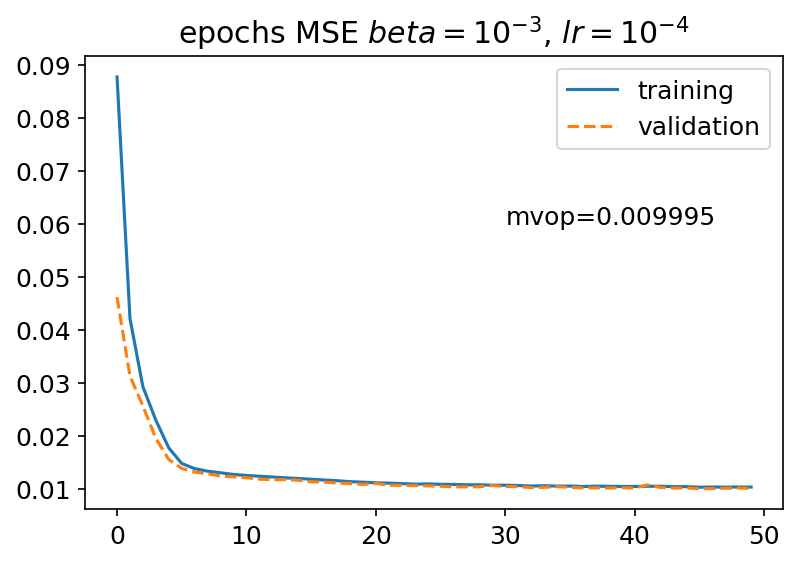
\includegraphics[height=4.5cm]{img/STEP1/training_20-20-10-10_b1e-3.png}    \label{fig:step1_regularization_e3}}
    \subfigure{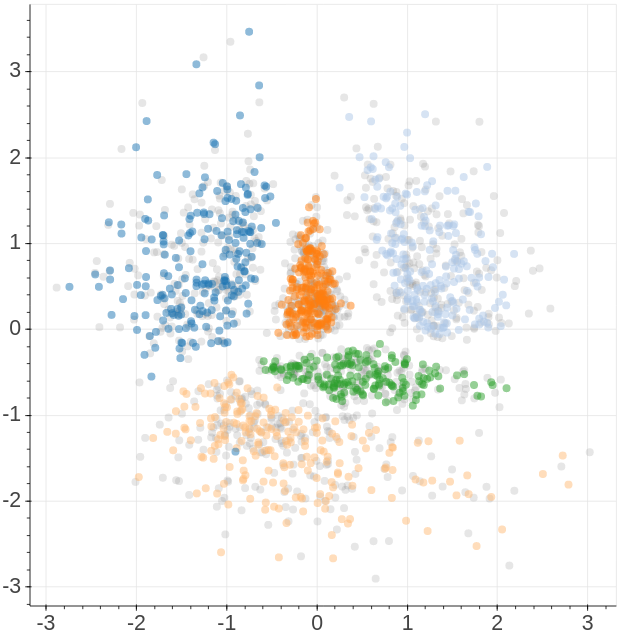
\includegraphics[height=4.5cm]{img/STEP1/training_20-20-10-10_b1e-3_ls.png} \label{fig:step1_regularization_e3_ls}}
    \subfigure{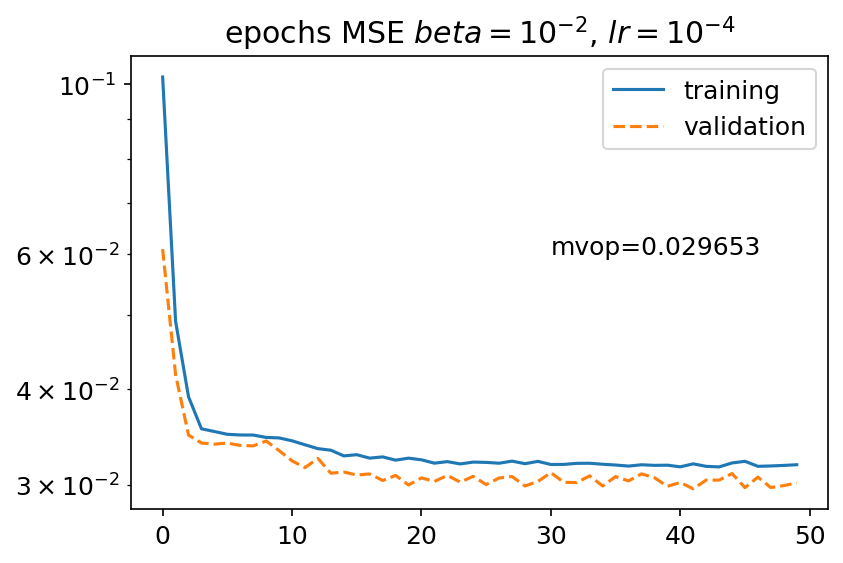
\includegraphics[height=4.5cm]{img/STEP1/training_20-20-10-10_b1e-2_log.png}\label{fig:step1_regularization_e2}}
    \subfigure{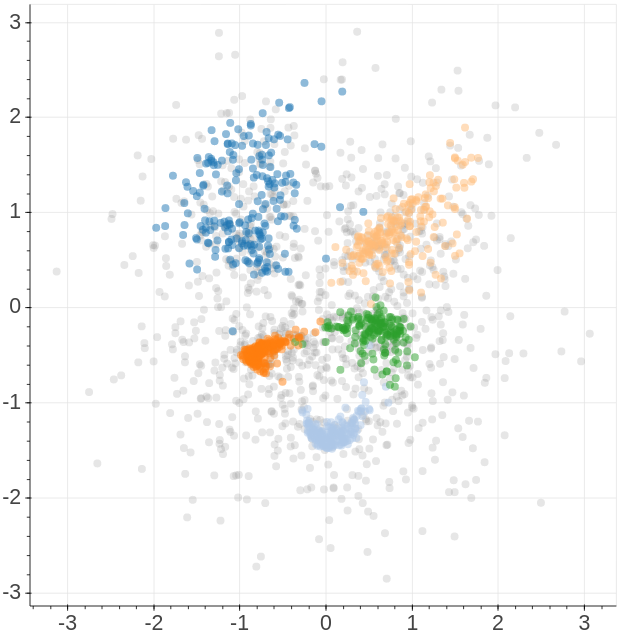
\includegraphics[height=4.5cm]{img/STEP1/training_20-20-10-10_b1e-2_ls.png} \label{fig:step1_regularization_e2_ls}}
    \caption{ Latent space regularization } 
    \label{fig:step1_ls_regularization}
\end{figure}
%
We adopted this solution, because it is very easy to be implemented in the \acs{VAE} code, being a simple additional loss factor in the KL addendum. Also it has been proved in~\cite{Higgins2017betaVAELB} to produce an effect comparable with other more complex approaches specifically designed for encouraging disentanglement such as InfoGAN~\cite{NIPS2016_6399} or DC-IGN~\cite{kulkarni2015deep}. 
In \Figure{\ref{fig:step1_ls_regularization}} two examples of training from the simulated signals are presented; where the loss per epoch is shown for both the training and validation, and the resulting scattering plot of the latent space for two possible $\beta$ selections.
Seen by the latent space the effect of disentangling factors reflects to a more compact clusters representation. While, from the topological point of view, the graph of the dual Voronoi diagram representation assumes a structure with edges that tends to align with the plot axes, meaning that a single variable is more capable to discriminate the generator classes.
However this comes with a price that is spent by the generator that loose precision in data reconstruction.

\subsection{Noise rejection}
Beside all possible refinements that can be added and are targeted to a better understanding of the latent space, \acs{VAE} can be considered also a robust solution to handle noisy or missing data. Indeed the sole activation of a portion of the network in case of missing covariates, and the recovering of feature from added noise is an outstanding result of the autoencoder. In \Figure{\ref{fig:step1_noise_rejection}} a successful example of both missing data and noise recovery is shown for an instance of the class $k_3$ of the example in \cref{section: gaussian sum generator}. The plot on the left shows with blue ($\bullet$) and a dashed curve an instance of the generator, while the orange ($\times$) are the same set where missing values and noise have been applied. From the original set half of the measures has been removed and a Gaussian noise with $\sigma=3\times10^{-2}$ has been added. The green line with ($+$) is the resulting decoder output form a \VAE{2}, and it can be seen that it matches the original signal. On the right of the same figure the latent space is plotted for several samples in grey, a blue dot identifies the position of the original curve in latent coordinates, while the orange is the position of the reconstructed one, showing the fit error in latent space.
\begin{figure}
    \centering
    \subfigure[]{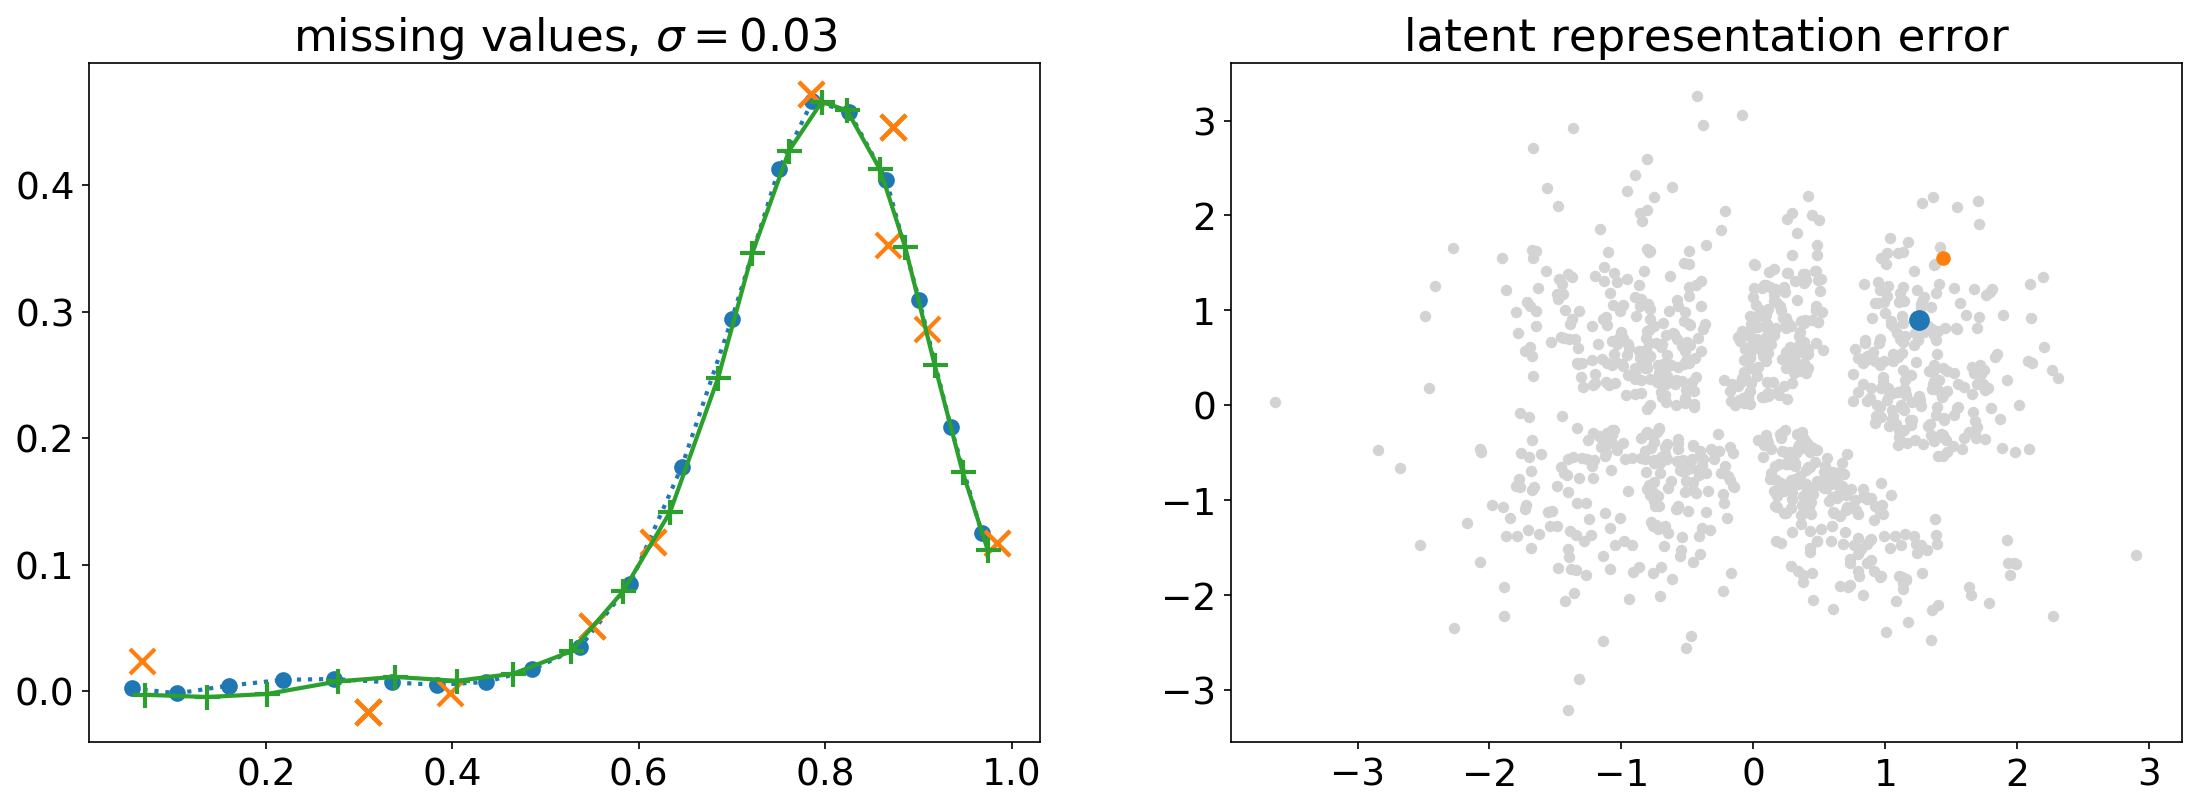
\includegraphics[height=4.5cm]{img/STEP1/recover_noise_err1.png} \label{fig:step1_noise_rejection}}
    \subfigure[]{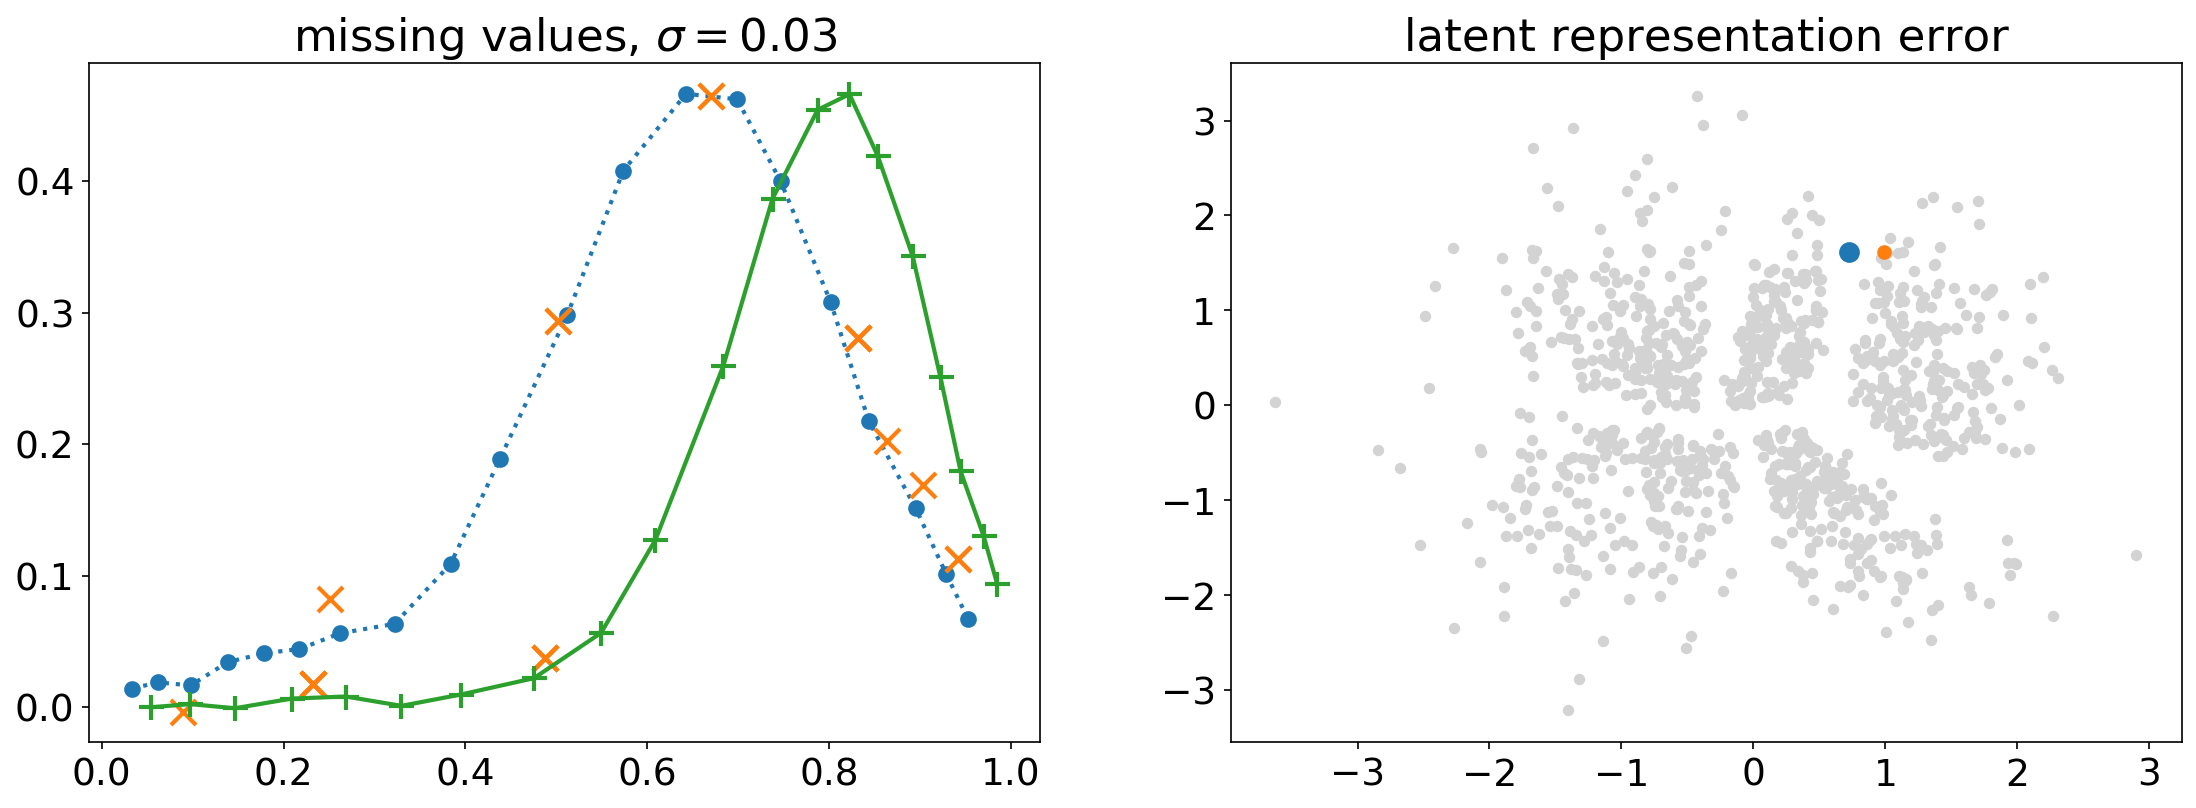
\includegraphics[height=4.5cm]{img/STEP1/recover_noise_err2.png} \label{fig:step1_noise_rejection_failed}}
    \caption{ Noise rejection } 
    \label{fig:step1_noise}
\end{figure}
Although the fitting behavior of the simple \VAE{2} model seems to provide an impressive precision in noise rejection, in this case a careful evaluation on the produced output should be also considered. A clear example is a failed reconstruction from noisy data shown in \Figure{\ref{fig:step1_noise_rejection_failed}}: here a curve has been created by the generative network itself by selecting a specific point in the boundary between two classes, to have a critical set of covariates that are not in the training dataset. Then the same noise and missing values of the previous example have been applied as it were a normal input. \VAE{2} in this case applies a recovery of the noise preferring to match a curve that matches a small amount of input data (i.e. the three orange crosses on the lower right) because those noisy values are compatible with a specific class of curves so it is more likely to be in the original training dataset.





\section{Other Kinds of Networks}

%   ____    _    _   _ 
%  / ___|  / \  | \ | |
% | |  _  / _ \ |  \| |
% | |_| |/ ___ \| |\  |
%  \____/_/   \_\_| \_|
%
\subsection{Generative Adversarial Networks}
%
Like the previously described Autoencoders, the Generative Adversarial Networks~\cite{goodfellow2014generative} belong to the generative models family, meaning that they are able to generate new "unseen" content. The overall framework of GAN is quite similar to what has been previously explained; there are both the encoder section and the decoder that are respectively used as inference and generator networks; however the inference is actually leading not to an output multidimensional space but directly to a binary value that is eventually trained to tell whether the input feature is coming from unseen external data or it has been generated by the included decoder.

Because of this binary classification behavior, the inference net in GANs is referred as the \textit{discriminator} and it is not meant to be of any use except to provide a backpropagation error in all the cases where a generated output is distinguishable from an input feature. In this way the training action is again twofold: the optimization of the encoder network that learns how to distinguish features from fakes, and the generator that is trained to produce samples from the posterior.

The generative action in GANs is performed by a classical decoder network, where we start from a opportunely shaped array of random variables to generate output. Here is the analogy with VAEs: the generation starts from a random vector that usually is characterized by a uniform distribution, likewise the generated input the VAE reparametrization step. However in this case we feed this randomly generated vector directly in the generator, without shaping the latent space with respect to the features, i.e. without reconstructing the posterior of the latent distribution conditioned on features.

This new approach comes with advantages and disadvantages. 
%
The disadvantages are primarily due to the just mentioned lack of an explicit representation of $p(\bm{x})$; also the \textit{discriminator} must be well synchronized with the \textit{generator} during training (in particular, \textit{generator} must not be trained too much without updating the \textit{discriminator}).
%
Among the advantages there is the fact that gradients can be obtained directly from back-propagating the classification error, but no actual inference is needed during learning, and a wide variety of functions can be incorporated into the model.
Anyway the most widely assumed advantage of adversarial networks is that they generate very sharp, even degenerate, distributions; while methods that are Markov based (i.e. comes from a bayesian network, like in the case of Variational Autoencoders) require the distribution to be somewhat blurry in order for the net to be able to mix between modes.
A worth to mention fact related to GAN is that they have proved to produce a disentangled representation, once a particular technique has been applied, called InfoGAN~\cite{NIPS2016_6399}, that at the beginning drew much attention toward them, since the $\beta$-VAE reconstruction proved to have almost the same disentangling benchmark.
%
Among the disadvantages there is also the fact that the training has slack information on the error being the sole classification result, so the it is used to present very slow convergence and the shape of input space has no structured manifold.

Although we implemented the GAN model within this research, studying the results has been quite discouraging with respect to VAE. Furthermore in this situation we miss some of the possible connections among models that we exploited in the next chapters and that require a fully working encoder to obtain the latent space.
Nevertheless GAN could remain a good diagnostic to diagnostic mapping, i.e. in our case scenario, imposing one diagnostic or parameter output as the latent input of generative network where we have it as a label for the target mapped diagnostic.
This could result quite opaque at this level, but it will be discussed in the conclusions when all elements of the study will have been exposed.


\subsection{Recurrent Neural Networks}
The defined network topology called \acl{RNN} is ultimately an order dependent network regularization of the basic perceptron. The vanilla \acs{MLP} takes its inputs in a fixed size vector that restricts the analysis to the finite size ergodic signal. On the other hand, the \acs{RNN} is a topology extension that exposes to the input features the network internal state, giving a chance for the model to interpret non-ergodic input windows, and with no predetermined limit in size. \acs{RNN}s take one or many input vectors and produce one or many output vectors in which the output is conditioned not only by direct inputs response, but also by a \textit{hidden state} that represents the current context where the input is evolving. In this way, the same input could produce different outputs depending on internal states, and, in turn, on the previous seen input. Nonetheless, this ordered sequence of the input covariates is not necessarily time dependent, for example the recurrency could be defined to implement the context analysis of a text.
%
% RR
For supervised learning in discrete time settings, sequences of real-valued input vectors arrive at the input nodes, one vector at a time. At any given time step, each non-input unit computes its current activation (result) as a nonlinear function of the weighted sum of the activations of all units that connect to it. Supervisor-given target activation can be supplied for some output units at certain time steps. For example, if the input sequence is a speech signal corresponding to a spoken digit, the final target output at the end of the sequence may be a label classifying the digit.

An \textit{Elman network} is a three-layer perceptron with the addition of a set of \textit{context} units. The middle (hidden) layer is connected to these context units fixed with a unitary weight. At each step the input is fed forward and the fixed backward connections save the previous values of the hidden units in the context ones. In this way the network maintains its inner state:
\begin{align}
    & \bm{x}_t = \sigma_x\left( A\bm{x}_{t-1} + B\bm{u}_t + \bm{w}_t \right) \\
    & \bm{y}_t = \sigma_y\left( C\bm{x}_t + \bm{v}_t \right)
    \label{eq:elman_model}
\end{align}
Similarly the output signal can be used as the inner state as well, in this case the topology structure is referred as the \textit{Jordan} recurrent network:
\begin{align}
    & \bm{x}_t = \sigma_x\left( A\bm{y}_{t-1} + B\bm{u}_t + \bm{w}_t \right) \\
    & \bm{y}_t = \sigma_y\left( C\bm{x}_t + \bm{v}_t \right)
    \label{eq:jordan_model}
\end{align}

% %% LSTM %%
% \subsubsection{LSTM}

% \section{Constraining regularizer with semi-supervised training}























